%%
%% This is file `sample-sigconf.tex',
%% generated with the docstrip utility.
%%
%% The original source files were:
%%
%% samples.dtx  (with options: `sigconf')
%%
%% IMPORTANT NOTICE:
%%
%% For the copyright see the source file.
%%
%% Any modified versions of this file must be renamed
%% with new filenames distinct from sample-sigconf.tex.
%%
%% For distribution of the original source see the terms
%% for copying and modification in the file samples.dtx.
%%
%% This generated file may be distributed as long as the
%% original source files, as listed above, are part of the
%% same distribution. (The sources need not necessarily be
%% in the same archive or directory.)
%%
%%
%% Commands for TeXCount
%TC:macro \cite [option:text,text]
%TC:macro \citep [option:text,text]
%TC:macro \citet [option:text,text]
%TC:envir table 0 1
%TC:envir table* 0 1
%TC:envir tabular [ignore] word
%TC:envir displaymath 0 word
%TC:envir math 0 word
%TC:envir comment 0 0
%%
%%
%% The first command in your LaTeX source must be the \documentclass
%% command.
%%
%% For submission and review of your manuscript please change the
%% command to \documentclass[manuscript, screen, review]{acmart}.
%%
%% When submitting camera ready or to TAPS, please change the command
%% to \documentclass[sigconf]{acmart} or whichever template is required
%% for your publication.
%%

\documentclass[sigconf]{acmart}


\usepackage{tikz}
\usepackage{tikz-network}
\usepackage{xspace}
\usepackage{xargs}
\usepackage[
  colorinlistoftodos,
  prependcaption,
  % disable,
]{todonotes}
\usepackage{fontenc}

%\usepackage{minted}

\usepackage{subcaption}

\usepackage{hyperref}


% !TEX root = ../main.tex

\usepackage{docmute}
\usepackage{hyperref}
\usepackage{proof}

\usepackage{mathtools}
\usepackage{tikz}
\usepackage{tikz-network}
\usepackage{xspace}
\usepackage{xargs}
\usepackage{fontenc}

%\usepackage{minted}

\usepackage{subcaption}
\usepackage{caption}

\usepackage{tikz-cd}
\usepackage{tikzit}
% to reduce tikz picture white space
\usepackage{adjustbox}

% for quotienting
\usepackage{xfrac} 

\usepackage{import}

% category names
%\newcommand{\MdaCospans}{{\catname{MACsp_{D}(Hyp_{\Sigma})}}}

\newcommand\HypI[1]{\textbf{HypI}(#1)}
\newcommand\MdaCospans{\textbf{MHypI}(\Sigma)}
\newcommand{\Ecospans}{{\catname{EHypI(\Sigma)}}}
\newcommand{\MdaEcospans}{{\catname{MEHypI(\Sigma)}}}
\newcommand{\WellTypedMdaEcospans}{{\catname{MEHypI(\Sigma)}}}
% conflict
\newcommand{\hashtag}{{\#}}
\newcommand{\consistency}{{\smile}}
% There is already a remark in the preamble, but it does
% not work for some reason
\newtheorem{remark}{Remark}


\usepackage{xifthen}
\ifthenelse{\isundefined{\ismain}}{
  \newcommand{\ismain}{0}
}{}

\usepackage{enumitem}
 
\newcommand{\ignora}[1]{ }

\ignora{
\usepackage{aliascnt}
% alias-counters
\newaliascnt{definition}{thm}
\newaliascnt{proposition}{thm} 
\newaliascnt{lemma}{thm}
\newaliascnt{corollary}{thm}
\newaliascnt{conjecture}{thm}
\newaliascnt{remark}{thm}
\newaliascnt{example}{thm}
\newaliascnt{examples}{thm}
\newaliascnt{assumption}{thm}
\newaliascnt{construction}{thm}
\newaliascnt{claim}{thm}

% \theoremstyle{plain}
\theoremstyle{definition}

\newtheorem{theorem}[thm]{Theorem}
\newtheorem{proposition}[proposition]{Proposition} 
\aliascntresetthe{proposition}
\newtheorem{lemma}[lemma]{Lemma}
\aliascntresetthe{lemma}
\newtheorem{corollary}[corollary]{Corollary}
\aliascntresetthe{corollary}
\newtheorem{conjecture}[conjecture]{Conjecture}
\aliascntresetthe{conjecture}
\newtheorem{remark}[remark]{Remark}
\aliascntresetthe{remark}
\newtheorem{assumption}[assumption]{Assumption}
\aliascntresetthe{assumption}
\newtheorem{construction}[construction]{Construction}
\aliascntresetthe{construction}
\newtheorem{claim}[claim]{Claim}
\aliascntresetthe{claim}

\theoremstyle{definition}
\newtheorem{definition}[definition]{Definition}
\aliascntresetthe{definition}
\newtheorem{example}[example]{Example}
\aliascntresetthe{example}
\newtheorem{examples}[examples]{Examples}
\aliascntresetthe{examples}
}

\usepackage{cleveref} % after hyperref!
% possibly new thm environment
% \newtheorem{satz}[thm]{Satz}


% \newcommand{\TODO}[1]{{{\color{red}[\textbf{TODO:} #1]}}}
% \newcommand{\TODO}[1]{}

% !TEX root = ../main.tex

\newcommand{\missing}[1]{{\color{red}\bfseries [TODO]}}

\newcommand{\egg}{\texorpdfstring{\MakeLowercase{\texttt{egg}}}{\texttt{egg}}\xspace}
\newcommand{\Egg}{\texorpdfstring{\MakeLowercase{\texttt{egg}}}{\texttt{egg}}\xspace}
% \newcommand{\egg}{Lego\xspace}
% \newcommand{\Egg}{Lego\xspace}
\newcommand{\egraphs}{\mbox{e-graphs}\xspace}
\newcommand{\egraph}{\mbox{e-graph}\xspace}
\newcommand{\Egraph}{\mbox{E-graph}\xspace}
\newcommand{\Egraphs}{\mbox{E-graphs}\xspace}
\newcommand{\eclass}{\mbox{e-class}\xspace}
\newcommand{\Eclass}{\mbox{E-class}\xspace}
\newcommand{\enode}{\mbox{e-node}\xspace}
\newcommand{\eclasses}{\mbox{e-classes}\xspace}
\newcommand{\enodes}{\mbox{e-nodes}\xspace}
\newcommand{\Enodes}{\mbox{E-nodes}\xspace}
% \newcommand{\regraph}{Regraph\xspace}
% \newcommand{\Regraph}{Regraph\xspace}
\newcommand{\sz}{Szalinski\xspace}
\newcommand{\find}{\texttt{find}\xspace}

\newcommand{\equivid}{\equiv_{\sf id}}
\newcommand{\equivnode}{\equiv_{\sf node}}
\newcommand{\equivterm}{\equiv_{\sf term}}

\newcommand{\congrinv}{$\mathcal{I}_c$\xspace}

\newcommand{\egglogo}[1][]{\protect\includegraphics[height=1em, #1]{egg.png} }
\newcommand{\eggurl}{\url{https://github.com/mwillsey/egg}}

% TODOs
% https://tex.stackexchange.com/questions/9796/how-to-add-todo-notes

\newcommand{\eggtodo}[1]{\textcolor{Red}{\textbf{[CITE: #1]}}}

\newcommand{\defTodo}[2]{%
  \expandafter\newcommand\csname #1\endcsname[1]{%
    \todo[linecolor=#2,backgroundcolor=#2!25,bordercolor=#2,inline,size=\tiny]{\textbf{#1}: ##1}}}

\newcommand{\defTODO}[2]{%
  \expandafter\newcommand\csname #1\endcsname[1]{%
    \todo[linecolor=#2,backgroundcolor=#2!25,bordercolor=#2,inline,size=\tiny,caption={\textbf{(#1 LONG TODO)}}]{##1}}}

\newcommand{\AlekseiColor}{RoyalBlue}

% examples
% \newcommand{\RemyColor}{Red}
% \newcommand{\OliverColor}{OliveGreen}
% \newcommand{\ChandraColor}{Magenta}
% \newcommand{\PavelColor}{Cerulean}
% \newcommand{\ZachColor}{Plum}
% \newcommand{\BenColor}{Orchid}
% \newcommand{\JamesColor}{Salmon}


\defTodo{Aleksei}{\AlekseiColor}
% \defTodo{Max}{\MaxColor}

\defTODO{ALEKSEI}{\AlekseiColor}
% \defTODO{MAX}{\MaxColor}


% categorical stuff

\newcommand{\catname}[1]{\mathbf{#1}}

\newcommand{\Graph}{\catname{Graph}}
\newcommand{\Set}{\catname{Set}}

\newcommand\id{\textsf{id}}
\newcommand\sym{\textsf{sym}}

% tiny inline string diagrams
\newcommand{\comonoid}{%
	\begin{tikzpicture}[baseline=0.4ex, scale=0.4, line width=0.8pt]
		\path [use as bounding box] (0,0) rectangle (0.6,0.8);
		\draw (0.2,0) -- (0.2,0.4);
		\filldraw[black] (0.2,0.4) circle (0.08);
		\draw (0,0.8) .. controls (0,0.65) and (0.1,0.45) .. (0.2,0.4);
		\draw (0.4,0.8) .. controls (0.4,0.65) and (0.3,0.45) .. (0.2,0.4);
	\end{tikzpicture}%
}
\newcommand{\counit}{%
	\begin{tikzpicture}[baseline=0.4ex, scale=0.4, line width=0.8pt]
		\path [use as bounding box] (0,0) rectangle (0.4,0.8);
		\draw (0.2,0) -- (0.2,0.4);
		\filldraw[black] (0.2,0.4) circle (0.08);
	\end{tikzpicture}%
}

% camera-ready
\newcommand{\ifcameraready}[2]{\ifdefined\cameraready #2 \else #1 \fi}

\input{sample.tikzstyles}
\input{hypergraph.tikzstyles}
\input{hypergraph.tikzdefs}


\definecolor{applegreen}{rgb}{0.55, 0.71, 0.0}
\definecolor{americanrose}{rgb}{1.0, 0.01, 0.24}
\definecolor{atomictangerine}{rgb}{1.0, 0.6, 0.4}
\definecolor{azure}{rgb}{0.0, 0.5, 1.0}

% These are for comments
\newcommand\question[1]{{\color{azure}#1}}
\newcommand\update[1]{{\color{americanrose}#1}}

% \usepackage{mathtools,mathrsfs}
\usepackage{tikz-cd}
\usepackage{tikzit}

% for quotienting
% \usepackage{faktor}
\usepackage{xfrac} 

\usepackage{import}

% category names
%\newcommand{\MdaCospans}{{\catname{MACsp_{D}(Hyp_{\Sigma})}}}

\newcommand\HypI[1]{\textbf{HypI}(#1)}
\newcommand\MdaCospans{\textbf{MHypI}(\Sigma)}
\newcommand{\Ecospans}{{\catname{EHypI(\Sigma)}}}
\newcommand{\MdaEcospans}{{\catname{MEHypI(\Sigma)}}}
\newcommand{\WellTypedMdaEcospans}{{\catname{WMEHypI(\Sigma)}}}
% conflict
\newcommand{\hashtag}{{\#}}
\newcommand{\consistency}{{\smile}}
% There is already a remark in the preamble, but it does
% not work for some reason
\newtheorem{remark}{Remark}

\makeatletter
\newsavebox{\@brx}
\newcommand{\llangle}[1][]{\savebox{\@brx}{\(\m@th{#1\langle}\)}%
  \mathopen{\copy\@brx\kern-0.5\wd\@brx\usebox{\@brx}}}
\newcommand{\rrangle}[1][]{\savebox{\@brx}{\(\m@th{#1\rangle}\)}%
  \mathclose{\copy\@brx\kern-0.5\wd\@brx\usebox{\@brx}}}
\makeatother


%%
%% \BibTeX command to typeset BibTeX logo in the docs
\AtBeginDocument{%
  \providecommand\BibTeX{{%
    Bib\TeX}}}

%% Rights management information.  This information is sent to you
%% when you complete the rights form.  These commands have SAMPLE
%% values in them; it is your responsibility as an author to replace
%% the commands and values with those provided to you when you
%% complete the rights form.
\setcopyright{acmlicensed}
\copyrightyear{2024}
\acmYear{2024}
\acmDOI{XXXXXXX.XXXXXXX}

%% These commands are for a PROCEEDINGS abstract or paper.
\acmConference[LICS '24]{Logic in Computer Science}{July 8--12,
  2024}{Tallinn, Estonia}
%%
%%  Uncomment \acmBooktitle if the title of the proceedings is different
%%  from ``Proceedings of ...''!
%%
%%\acmBooktitle{Woodstock '18: ACM Symposium on Neural Gaze Detection,
%%  June 03--05, 2018, Woodstock, NY}
\acmISBN{978-1-4503-XXXX-X/18/06}


%%
%% Submission ID.
%% Use this when submitting an article to a sponsored event. You'll
%% receive a unique submission ID from the organizers
%% of the event, and this ID should be used as the parameter to this command.
%%\acmSubmissionID{123-A56-BU3}

%%
%% For managing citations, it is recommended to use bibliography
%% files in BibTeX format.
%%
%% You can then either use BibTeX with the ACM-Reference-Format style,
%% or BibLaTeX with the acmnumeric or acmauthoryear sytles, that include
%% support for advanced citation of software artefact from the
%% biblatex-software package, also separately available on CTAN.
%%
%% Look at the sample-*-biblatex.tex files for templates showcasing
%% the biblatex styles.
%%

%%
%% The majority of ACM publications use numbered citations and
%% references.  The command \citestyle{authoryear} switches to the
%% "author year" style.
%%
%% If you are preparing content for an event
%% sponsored by ACM SIGGRAPH, you must use the "author year" style of
%% citations and references.
%% Uncommenting
%% the next command will enable that style.
%%\citestyle{acmauthoryear}

\begin{document}

\title{Equivalence Hypergraphs: E-Graphs for Monoidal Theories}

\author{Anonymous}
%\email{}
%\orcid{}
%\affiliation{
%  \institution{}
%  \streetaddress{}
%  \city{}
%  \state{}
%  \country{
%  \postcode{}
%}

%\renewcommand{\shortauthors}{}

\begin{abstract}
The technique of equipping graphs with an equivalence relation, called equality saturation, has recently proved both powerful and practical in program optimisation, particularly for SMT solvers. 
We give a categorical semantics to these structures, called \emph{e-graphs}, in terms of Cartesian categories enriched over a semilattice. 
We show how this semantics can be generalised to monoidal categories, which opens the door to new applications of e-graph techniques, from algebraic to monoidal theories.
Finally, we present a sound and complete combinatorial representation of morphisms in such a category, based on a generalisation of hypergraphs (\emph{e-hypergraphs}).
They have the usual advantage that many of their structural equations are absorbed into a general notion of isomorphism. 
\end{abstract}

%%
%% The code below is generated by the tool at http://dl.acm.org/ccs.cfm.
%% Please copy and paste the code instead of the example below.
%%

\begin{CCSXML}
<ccs2012>
   <concept>
       <concept_id>10003752.10010124.10010131.10010137</concept_id>
       <concept_desc>Theory of computation~Categorical semantics</concept_desc>
       <concept_significance>300</concept_significance>
       </concept>
   <concept>
       <concept_id>10003752.10003809.10010031</concept_id>
       <concept_desc>Theory of computation~Data structures design and analysis</concept_desc>
       <concept_significance>300</concept_significance>
       </concept>
   <concept>
       <concept_id>10002950.10003624.10003633.10003637</concept_id>
       <concept_desc>Mathematics of computing~Hypergraphs</concept_desc>
       <concept_significance>300</concept_significance>
       </concept>
   <concept>
       <concept_id>10003752.10003790.10003798</concept_id>
       <concept_desc>Theory of computation~Equational logic and rewriting</concept_desc>
       <concept_significance>300</concept_significance>
       </concept>
 </ccs2012>
\end{CCSXML}

\ccsdesc[300]{Theory of computation~Categorical semantics}
\ccsdesc[300]{Theory of computation~Data structures design and analysis}
\ccsdesc[300]{Mathematics of computing~Hypergraphs}
\ccsdesc[300]{Theory of computation~Equational logic and rewriting}

\keywords{e-graphs, categorical semantics, enriched category theory,  hypergraph rewriting,  DPO rewriting.}

%\received{20 February 2007}
%\received[revised]{12 March 2009}
%\received[accepted]{5 June 2009}

\newcommand\id{\textsf{id}}
\newcommand\sym{\textsf{sym}}

\maketitle

%-------------------- INTRODUCTION

\section{Introduction}


Rewrite-driven program optimisation consists of the application of a sequence of semantics-preserving rewrites which may improve the cost of execution, such as time or space (memory). 
Because the application of some rewrites can either enable or block the subsequent application of others, the choice of application order significantly impacts the quality of the resulting optimisation.  This long-standing issue is known as the \textit{phase-ordering problem}, with a \textit{phase} referring to a particular set of rewrites. Typical approaches to this problem use heuristics to determine an ordering. 

A recently proposed,  alternative solution is \textit{equality saturation} 
\cite{10.1145/1594834.1480915}: instead of maintaining a \textit{single},  putatively optimised program which is rewritten \textit{destructively} at each step, a \textit{set} of equivalent programs is maintained instead, whereas each rewrite step \textit{non-destructively} grows the set.  Upon reaching a fixed point (\textit{saturation}),  a \textit{globally} optimal program can then be extracted from this set.
A naive approach is clearly unfeasible, since the size of this set grows exponentially with the number of rewrites. 
However, \textit{equality graphs (e-graphs)} \cite{EggPaper} are a data structure that can represent this set compactly, thus making the set tractable in practical applications. 

Although equality saturation is already a state-of-the-art algorithmic optimisation technique, there is an opportunity to better understand its mathematical foundations. 
We propose to address this issue via a categorical axiomatisation for e-graphs and their rewriting. 
Considering programs as represented by terms of an arbitrary algebraic theory, we demonstrate a correspondence between e-graphs and (string diagrams for) simple \textit{semilattice-enriched} Cartesian categories. 
The approach we take is guided by the established methodology of creating a correspondence between string diagrams and graph rewriting, as encountered in a large body of research. 
The starting innovation of our approach is the semilattice-enrichment. 
The \textit{join} operator lifts the formalism so that it can now operate with \textit{sets} of terms (string diagrams, morphisms); the rest of the paper is about working out the mathematical implications of introducing this enrichment to string diagrams and their concrete combinatorial represetation. 

Although our primary interest is theoretical, we believe that phrasing e-graphs in the more general language of category theory will open the door to new potential domains of applications that now use string diagrams and which require the application of optimisation techniques \cite{Selinger_2010, Hasegawa-traced}. 
This may include areas as diverse as digital \cite{ghica_compositional_2023} and quantum circuits
\cite{coecke_interacting_2011,ZX}, functional programs~\cite{ghica_hierarchical_2023}, or computational linguistics \cite{wazni_quantum_2022,coecke_lambek_2013}.  
However, in this work we offer little to the e-graph practitioner, as we focus exclusively on foundational aspects, introducing no new applications or improved e-graph algorithmics. 

A final contribution of this work is giving a concrete combinatorial representation of enriched string diagrams in terms of (hierarchical)  hypergraphs, which we call \textit{e-hypergraphs}.  We also give a specification of e-hypergraph rewriting via a suitable extension of the double pushout (DPO) rewriting framework 
\cite{dpo, bonchi_string_2022-1,bonchi_string_2022-2,bonchi_string_2022},  proving the representation \textit{sound and complete} with respect to our categorical semantics.  As a corollary, this also provides a formalisation of the rewriting theory of e-graphs as encountered in the literature. 

\subsection{E-graphs}


\begin{figure*}\label{fig:e-graph-example}
\[
	\hspace{1.3cm}
    \scalebox{0.65}{
    \tikzfig{categorical-semantics/egraph-translation}
    }
\]
\caption{Example translation of acyclic e-graphs into string diagrams for semilattice enriched Cartesian categories. }
\end{figure*}

E-graphs are a data structure which can efficiently represent many equivalent terms of an algebraic theory.  They generalise the typical DAG representation of terms to include equivalence classes. 
The key concepts of e-graphs can be intuitively grasped from some simple (but non-trivial) examples, as shown in Figure~\ref{fig:e-graph-example}.
This example is a `Hello world!' of e-graphs, presented first in~\cite{EggPaper}.

Each column represents a term (or term rewrite rule), the conventional e-graph representation, and the equivalent e-string diagram representation, an e-hypergraph. 
The initial term, $(a*2)/2$, is already represented efficiently in the e-graph by sharing the node 2.
The string diagram version is slightly different than conventional e-graphs by representing the sharing of the node 2 explicitly, using a sharing (contraction) node. 

Nodes are encapsulated in dashed boxes indicating equivalence classes of nodes, or, more generally, of subgraphs. 
Initially each equivalence class has a single node. 
The first rewrite rule, replacing multiplication by the more efficient \emph{shift-left} operator creates the first non-unitary equivalence class, which includes the multiplication ($*$) and shift-left ($<\!\!<$) operator nodes, with a new sharing, that of node $a$. 
This second e-graph illustrates the other difference, besides sharing, between conventional e-graphs and e-hypergraphs, namely the fact that in the former edges connect directly to nodes inside the equivalence class, whereas in the latter edges connect to the equivalence class itself. 
Explicit discarding (weakening) nodes indicate which of the class-level edges are connected to which nodes inside the class. 

The other steps, (c) to (e), represent further elaborations of the e-graph, or e-hypergraph, via the application of more rules. 
Note that in the final e-graph, (e), a cycle is introduced, making it the representation of infinitely many terms: $a, a*1, (a*1)*1, \ldots$. 
From the saturated graph the optimal term consisting of only the node $a$ can be then extracted, discarding everything else. 

\subsection{Semilattice Enriched Categories}

\begin{figure}
\[
	\scalebox{0.65}{
	\tikzfig{categorical-semantics/egraph-strings}
	}
\]
\caption{String diagrams for semilattice enriched symmetric monoidal categories.}
\end{figure}\label{fig:egraph-strings}

Recalling the correspondence between DAG representations of algebraic terms and  string-diagrams for morphisms of a suitable Cartesian category
makes perspicuous the correspondence between (acyclic) e-graphs and morphisms of a suitably enriched Cartesian category, taken as string diagrams~\cite{noauthor_09083347_nodate,joyal_geometry_1991, mellies_functorial_2006}. We extend the usual vocabulary of string diagrams for symmetric monoidal categories with the additional generator  
\[
\infer{\phi_1 + \ldots + \phi_n: A \to B}{\{\phi_i: A \to B\}_{i \in \{1,\ldots,n\}}}
\]
The ability to take formal (non-empty) joins of morphisms is used to model the equivalence class structure of e-graphs.  

String diagrams are read from bottom-to-top; we consider additional generators for the duplication and deletion transformations of a Cartesian category.  Note, further, that in the Cartesian case we can restrict to generating morphisms $c$ to have a single output,  without loss of generality,  by applying the universal properties of the Cartesian product.  This means the (informal) translation given below is fully general for acyclic e-graphs. 

The translation from e-graphs to enriched string diagrams is illustrated informally below,
noting how the typing constraints of the $+$ constructor are satisfied in the image of the translation by discarding in each component all unnecessary inputs.
\[
    \tikzfig{categorical-semantics/egraph-translation-1}
\]
Examples of this translation are given in the second row of Figure \ref{fig:e-graph-example}. In particular, note that the translation of the \textit{cyclic} e-graph (e)
requires the use of a categorical \textit{trace}, generating a cycle. In this paper, we focus on \textit{acyclic} e-graphs and their corresponding catgeories; but the above example illustrates that the extension to the cyclic case seems to be routine. As it would involve needless additional presentational complexity we leave it as further work. 

Note that the motivating example of our work, e-graphs, requires the Cartesian structure. 
However, we will see how all the core of the theory of e-hypergraph rewriting only requires the monoidal structure. 
Thus we can readily generalise e-graphs from algebraic to monoidal theories, giving rise to a  host of new potential applications, which we briefly outline in the conclusion of this paper.   

\subsection{Combinatorial Representation of Enriched String Diagrams}

In order to \textit{implement} generalised e-graphs, rewriting must be performed on concrete representations of the corresponding string diagrams.  String diagrams can be considered equivalently as either topological objects (\textit{i.e.}, taken modulo ``connectivity'') or as a 2-dimensional syntax quotiented by the equations of an SMC. For example, we have the following equivalences between diagrams. 
%\[(f_1 \otimes f_2) ; (g_1 \otimes g_2) = (f_1 ; g_1) \otimes (f_2 ; g_2)\] 
\[
	\scalebox{0.6}{
	\tikzfig{categorical-semantics/interchange}
	}
\]
This representation makes string diagrams unamenable to efficient implementation due to the difficulty of calculating the quotient. 
A large body of research work shows how this issue can be solved by taking a different approach, representing string diagrams as hypergraphs~\cite{bonchi_string_2022-1,bonchi_string_2022-2,bonchi_string_2022}.  Here, the generators $c_i$ become vertices, connected via hyper-edges.  Thus the expected quotient becomes simply hypergraph isomorphism. With appropriate restrictions on the form these hypergraphs can take, this approach can be used to \textit{characterise} the free symmetric monoidal category generated by some~$c_i$. 

We are interested not only in the free SMC over a set of generators, but also in \textit{(symmetric) monoidal theories} with extra equations such as, for instance, the rewrite rules (b)--(e) of Figure \ref{fig:e-graph-example}. These can be seen as equations between string diagrams, and thus rewrites of their hypergraph representations.  Because the generating equations can be applied in any context, we are lead to the notion of \textit{(hyper)graph rewriting}: given an equation $l=r$, we require some way to identify (a sub-hypergraph corresponding to) $l$ in any hypergraph $G$ and replace it with (a sub-hypergraph corresponding to) $r$.
The standard methodology to giving specifications of such graph rewriting, known as \textit{double pushout (DPO) rewriting} \cite{???} is still applicable.
However, these concepts must be now generalised from hypergraphs to \textit{e-hypergraphs}, hypergraphs with two additional relations denoting the hierarchical structure introduced by so-called \textit{e-boxes}: the generator for semilattice enrichment, and the separation of the components of each e-box.
Giving the appropriate definitions turns out to be a technical matter of some complexity, and constitutes the main body of the paper. 

\subsection{Soundness and Completeness}
The main technical result of the paper is a proof of soundness and completeness of the combinatorial representation for semilattice enriched SMCs, extending the results of \cite{bonchi_string_2022-2} for plain SMCs. While the structural equalities of SMCs are factored out in the representation,  important structural equalities arising from the enrichment (see the equations of Figure \ref{fig:string-equations}) are not, and should not be. They represent the un/sharing of subdiagrams with respect to the e-box structure,  which is precisely what allows for the compact representation of equivalence classes.  Instead, we consider DPO-rewrites implementing both the structural equalities for enrichment (which involve the e-box structure) and the equalities arising from the generating monoidal theory (which do not).  

Quotienting e-hypergraphs by the induced equivalence gives rise to a sound and complete model of semilattice enriched SMCs.  That is, we exhibit a translation functor $\llbracket-\rrbracket$ from the free semilattice enriched SMC over a symmetric monoidal theory to our (quotiented) category of e-hypergraphs such that 
morphisms $f = g$ if and only if there exists a sequence of DPO-rewrites (each induced by a structural equality or the monoidal theory) between their translations: $\llbracket f \rrbracket \rightsquigarrow_{DPO} \llbracket g \rrbracket$. 

DAN: THIS NEEDS EXPANDING. EXPLAINING IN PLAIN WORDS SOME OF THE THEORETICAL PROPERTIES OF E-GRAPHS AND THE CATEGORICAL STATEMENT. 

%\subsection{E-matching and E-rewriting}
%
%Having defined e-hypergraphs and shown them to correctly model the rewriting of string diagrams for semilattice enriched SMCs, we note that the naive implementation of DPO-rewriting is inefficient: to find a redex within an e-hypergraph involves finding a structurally equivalent e-hypergraph which contains the redex as a subgraph. In general, this involves unsharing the e-box structure before a redex becomes available.  Thus, we define a notion of \textit{e-matching} for e-hypergraphs: that is, to find redexes working modulo the e-box structure. In particular, we wish to locate the smallest subgraph $G' \subseteq G$ "containing" (in an appropriate sense) the redex $L$. Given this,  \textit{e-rewriting} $L \to R$, intended to achieve equality saturation, is simple to define due to its non-destructive nature: we rewrite $G' \to G' + R$ in $G$.  
%\begin{figure}
%\[
%	\tikzfig{combinatorial_semantics/example-rewriting}
%\]
%\caption{Example application of e-rewriting for rewrite $(x*y)/z \to x*(y/z)$: find an appropriate minimal sub-e-hypergraph containing the redex $(x*y)/z$ and non-destructively add the reduct $x*(y/z)$.  REDO THIS}
%\end{figure}

\subsection{Related Work}

Although e-graphs were first developed in the 80's \cite{nelson1980techniques}, there has recently been an explosion of interest in them for the purpose of building program optimisers and synthesisers, especially due to recent work on the equality saturation technique \cite{10.1145/1594834.1480915, griggio_proceedings_2022, EggPaper,flatt_small_2022}.  This includes interest in various extensions of the e-graph formalism, for example to account for conditional rewriting \cite{singher2023colored},  to reason about rewriting for the $\lambda$-calculus \cite{koehler2022sketchguided},  and to combine techniques of e-graphs and database queries (``relational e-matching'') \cite{zhang_relational_2022}.  We are hopeful that our novel perspective on e-graphs can be extended to give uniform foundations to these investigations.  Some further avenues for investigation, including potential applications, are given in the conclusion of this paper. 

Our use of string diagrams is also central to the intuition behind our work.  There is a breadth of work on similar string diagrammatic formalisms,  including hierarchical string diagrams \cite{ghica_hierarchical_2023} and functorial boxes \cite{mellies_functorial_2006},  proof nets for compact closed categories with biproducts \cite{duncan_generalised_2009}, and recent work on tape diagrams for rig categories with biproducts \cite{bonchi_tape_nodate}. 

CHRIS: CITE HASEGAWA - TRACE MONOIDAL CATEGORIES, AND PERDIX. 
DAN: I SUGGEST TO CITE HASEGAWA IN FURTHER WORK, FOR GENERALISING THE THEORY TO TRACED MC.
DAN: THIS NEEDS TO BE CAREFULLY EXPANDED TO NOT OFFEND POTENTIAL REVIEWERS. 

\section{Categorical Semantics of E-Graphs}
In this section,  we introduce the required preliminaries on semilattice enriched symmetric monoidal categories generated by monoidal theories,  and the string diagrammatic formalism we will use to represent them.  

Given a $\mathbb{C}$  with objects $A,B \in \mathbb{C}$ we denote by $\mathbb{C}(A,B)$ the corresponding hom-set.  We write the identity morphism on $A$ as $\id_A$,  or simply $A$.  We commonly write $f;g$ for composition in diagram order.  Composition in the usual order is written $g \circ f$.  We denote the tensor product of a \textit{symmetric monoidal category (SMC)} $\mathbb{C}$ by $\otimes$,  its unit by $1$ and its symmetry natural transformation as $\sym$ \cite{maclane}.  We adopt the convention that $\otimes$ binds more tightly than $(;\!)$.  We elide all associativity and unit isomorphisms associated with monoidal categories,  and often omit subscripts on identities and natural transformations where it can be inferred.  We denote by $\textsf{SLatt}$ the category of semilattices.  


\subsection{Symmetric Monoidal Theories and PROPs. }

A presentation of an algebraic theory is traditionally given by a \textit{signature} of $n$-ary operations and a set of \textit{equations}---formally,  pairs of terms freely generated over the signature.  We are interested here in symmetric monoidal theories, which are generalizations of algebraic theories where the operations of the signature may have arbitrary \textit{co-arities}.  First,  we generalize the notion of a signature. 
\begin{definition}[Monoidal signature]
A \textit{(monoidal) signature} $\Sigma$ is given by a set of \textit{generators} $f: n \to m$,  with \textit{arity} $n$ and \textit{coarity} $m$.  %A \textit{signature homomorphism} $h: \Sigma \to \Gamma$ is a function from $\Sigma$ to $\Gamma$ which preserves the (co-)arities of elements. 
\end{definition}

A categorical presentation of a monoidal signature is given by a freely generated products and permutations category.  
\begin{definition}[Products and permutations category]
A \textit{products and permutations category (PROP)} is a strict symmetric monoidal category with natural numbers as objects,  and such that $n \otimes m = n+m$.  A \textit{PROP functor} is a strict SMC-functor which is additionally identity-on-objects. 
We denote the free \textit{products and permutations category} over a monoidal signature $\Sigma$ by $\textbf{PROP}(\Sigma)$.  
\end{definition}
The free category $\textbf{PROP}(\Sigma)$ can be syntactically constructed from taking (typed) categorical combinator terms freely constructed from generators $f \in \Sigma$, $\textsf{id}_1$, $\sigma_{1,1}$, $(;\!)$ and $\otimes$, quotiented by the axioms of a symmetric monoidal category.  

An equation associated with a monoidal signature is a pair of parallel morphisms of the form above, leading to the following definition of a symmetric monoidal theory. 
\begin{definition}[Symmetric Monoidal Theory]
A \textit{presentation of a symmetric monoidal theory} $(\Sigma, \mathcal{E})$ is given by a pair of a monoidal signature $\Sigma$ and a set $\mathcal{E}$ of pairs of parallel morphisms $\phi,\psi: n \to m$ of $\textbf{PROP}(\Sigma)$.
A \textit{symmetric monoidal theory} $\textbf{SMT}(\Sigma,\mathcal{E})$ generated by a presentation $(\Sigma, \mathcal{E})$ is given by $\textbf{PROP}(\Sigma)$ quotiented by the least congruence including $\mathcal{E}$.
\end{definition}

It will often be convenient to give presentations of SMTs in terms of string diagrams.
\begin{example}
The SMT of \textit{commutative comonoids} is given by the following generators, ${\Delta, !}$, depicted in string diagrammatic form:
\[
	\scalebox{0.8}{
  	 \tikzfig{categorical-semantics/Cartesian-equipment}
	}
\]
together with the following associativity, commutativity and unitality equations, again given in terms of string diagrams. 
\[
	\scalebox{0.6}{
	\tikzfig{categorical-semantics/Cartesian-theory}	
	}
\]
The Cartesian SMT is given by a set of generators $\Sigma_C$, together with the generators and equations of the SMT of commutative monoids, and the following additional naturality equations, for every $c \in \Sigma_C$
\[
	\scalebox{0.6}{
	\tikzfig{categorical-semantics/Cartesian-naturality}
	}
\]
By Fox's Theorem~\cite{fox},  $\textbf{SMT}(\Sigma_C, \mathcal{E}_C)$ is equivalent to the free Cartesian category over $\Sigma_C$. 
\end{example}

\subsection{Free Semilattice Enrichment: Formal Joins}

We will use enrichment to axiomatize the e-box structure as the ``join" of two morphisms $f,g: A \to B$ as $f + g: A \to B$.\footnote{Note, in particular,  that semilattices do not require a unit for $+$. This is important, since, in any commutative monoid enriched category,  if there exists a categorical product, then it must be a categorical biproduct \cite{maclane} ---a degeneracy we wish to avoid.} More precisely our hom-sets will be given the structure of a semilattice.  
Generally,  we may define a category \textit{enriched} in any other monoidal category $M$ (\textit{e.g.},  \textbf{SLatt}).  In this case,  hom-sets are generalized to hom-objects of $M$ (\textit{e.g.},  a semilattice) and composition 
\[
	\circ: Hom(B,C) \otimes Hom(A,B) \to Hom(A,C)
\]
is defined as a $M$-morphism.  In other words,  composition must respect the additional structure on hom-sets.  
In our case,  the category we wish to enrich is also monoidal,  so we additionally ask that the monoidal structure also respects this structure.  Technically, this amounts to asking that the tensor product is an enriched functor. 
We omit further details of the general case of enrichment here, and instead work with the following more concrete defintion, where $M = \textbf{SLatt}$.  

\begin{definition}[Semilattice-enriched PROP]
A \textit{semilattice enriched strict SMC (PROP)}  $\mathbb{C}$ is given by an SMC (PROP) $(\mathbb{C}, \otimes, 1,+)$ where every hom-set additionally has the structure of a semilattice $(\mathbb{C}(A,B), +)$ which respects the composition and tensor product in the following ways,  for all appropriately typed morphisms. 
\begin{align*}
f ; (g+h) &= f;g + f;h &
(f+g) ; h &= f;h + g;h \\
f \otimes (g+h) &= f \otimes g + f \otimes h & 
(f+g) \otimes h &= f \otimes h + g \otimes h,
%\item A set $ob(\mathbb{C})$ of objects;
%\item For every pair $A,B \in ob(\mathbb{C})$, a hom-semigroup $Hom(A,B)$;
%\item An element $\textsf{id}_{A,B} \in Hom(A,B)$; 
\end{align*}
Note,  we take $(;\!)$ and $\otimes$ to bind more tightly than $+$.
A \textit{semilattice enriched strict SMC (PROP) functor} $F: (\mathbb{C}, \otimes, 1,+) \to (\mathbb{D}, \otimes, 1,+)$ is given by a strict SMC (PROP) functor on the underlying SMCs (PROPs) which additionally satisfies $F(f+g) = F(f)+F(g)$.  We denote the \textit{freely enriched PROP (SMT)} over a monoidal signature $\Sigma$ as $\textbf{PROP}^+(\Sigma)$ ($\textbf{SMT}^+(\Sigma, \mathcal{E})$,  respectively). 
\end{definition}

The free category $\textbf{PROP}^+(\Sigma)$ can be syntactically constructed from taking (typed) categorical combinator terms freely constructed from generators $f \in \Sigma$, $\textsf{id}_1$, $\sigma_{1,1}$, $(;\!)$ and $\otimes$, as well as $f+g$, quotiented by the axioms of an enriched symmetric monoidal category.  

To aid reasoning, we introduce a new language of string diagrams for semilattice enriched SMCs, using a hierarchical ``box'' structure to capture the join operation on morphisms.  It was already discussed in the introduction how this is  used in the translation of equivalence classes from the e-graph to the string diagrammatic setting. 

Figure \ref{fig:egraph-strings} displays the generators of this language and Figure \ref{fig:string-equations} displays the additional equations which these diagrams satisfy, in addition to the standard SMC equations. 
We use string diagrams informally in this paper, but it is intuitively clear that these diagrams are sound and complete with respect to their intended categorical semantics. 
Indeed, similar diagrammatic languages using boxes to express choice have been used before~\cite{duncan_generalised_2009}. 

\begin{figure*}
\[  
    \scalebox{0.75}{
	\tikzfig{categorical-semantics/egraph-strings-equations}
    }
\]
\caption{Equations for a  semilattice enriched symmetric monoidal category}
\label{fig:string-equations}
\end{figure*}

\section{String Diagram Rewrite Theory}\label{sec:combinatorial-semantics}

In this section,  we recall the fundamental definitions and results of string diagram rewrite theory for symmetric monoidal categories,  building to the recapitulation of the correspondence between string diagram rewriting and an appropriate notion of double pushout (DPO) rewriting of certain hypergraphs,  as established in~\cite{Frobenius, Frobenius2}.  

First,  we fix some notation.  Let $(-)^*$ be the free monoid monad over \textsf{Set}.  
We extend this to the case of relations $R \subseteq V \times V$,  so that we denote by $R^{*} \subseteq V^* \times V^*$ the element-wise extension of $\psi$ to a relation on ordered sequences. 
We elide associativity and unit isomorphisms associated with coproducts $(+)$,  and denote by $\iota_j: X_{j} \rightarrow X_{1} + \ldots X_{j} + \ldots X_{n}$ the $j^{\text{th}}$ injection,  and $[f,g]: A_1 + A_2 \to B$ the co-pairing of two morphisms $f: A_1 \to B$ and $g:A_2 \to B$. 
We denote by $A +_{f,g} B$ the pushout of the span $A \xleftarrow{f} C \xrightarrow{g} B$.

\subsection{Hypergraphs}

In ~\cite{Frobenius},  hypergraphs \textit{with interfaces} and their DPO rewriting are shown to be sound and complete for SMTs including a Frobenius algebra. 
Hypergraphs generalize graphs by allowing edges to have multiple sources and targets. 
When interpreting string diagrams as hypergraphs,  morphisms are interpreted as edges,  and wires as vertices.  
However,  there is also a need to specify which vertices are to be considered as \textit{input} and \textit{outputs},  corresponding to the dangling wires at the bottom and top of a string diagram. 
This gives rise to the definition of a hypergraph with interfaces.  
Subsequent work \cite{Frobenius2} builds on this correspondence to give a restriction of hypergraphs with interfaces (called \textit{monogamous} directed acyclic),  leading to a correspondence between symmetric monoidal string diagrams and the category of such hypergraphs.


\begin{definition}[Category of hypergraphs]\label{def:hypergraph}
A \emph{hypergraph $\mathcal{G}$ over a signature $\Sigma$} is a tuple $(V,E,s,t,l)$,  where $V$ is a finite set of nodes, $E$ is a finite set of edges, $s : E \to V^{*}$ is a source function, $t : E \to V^{*}$ is a target function,  and $l : E \to \Sigma$ is a labelling function that assigns each edge a generator from monoidal signature $\Sigma$.  The labelling function must respect the typing of the generator: for all edges $e$,  $|s(e)| = m$ and $|t(e)| = n$,  where $l(e) : m \to n$. 
A \emph{hypergraph homomorphism} $\phi: \mathcal{F} \to \mathcal{G}$ is given by a pair of functions $\phi_V : V_{\mathcal{F}} \to V_{\mathcal{G}}, \phi_E : E_{\mathcal{F}} \to E_{\mathcal{G}}$ such that the following hold. 
\begin{enumerate}
    \item $\phi_V^*(s_{\mathcal{F}}(e)) = s_{\mathcal{G}}(\phi_E(e))$
    \item $\phi_V^*(t_{\mathcal{F}}(e)) = t_{\mathcal{G}}(\phi_E(e))$
    \item $l_{\mathcal{F}}(e) = l_{\mathcal{G}}(\phi_E(e))$
\end{enumerate}
We denote by $\catname{Hyp(\Sigma)}$ the category of hypergraphs over $\Sigma$.
\end{definition}
Note that $\catname{Hyp(\Sigma)}$ has all finite colimits and, in particular,  the coproduct is given by the disjoint union of hypergraphs.
The initial object is given by the empty hypergraph.  

\begin{definition}[Symmetric monoidal category of cospans]
Let $\mathbb{C}$ be a category with all finite colimits.  A cospan from $X$ to $Y$ is a pair of arrows $X \xrightarrow{} A \xleftarrow{} Y$  in $\mathbb{C}$.  This \textit{category of cospans of $\mathbb{C}$},  denoted $\catname{Csp(\mathbb{C})}$,  has as objects those of $\mathbb{C}$ and as arrows isomorphism classes of cospans.
%Two cospans $X \xrightarrow{} A \xleftarrow{} Y$ and $X \xrightarrow{} B \xleftarrow{} Y$ are isomorphic if the following diagram commutes and $\alpha$ is iso.
%\[
%\begin{tikzcd}
%                                               & A \arrow[dd, "\alpha"] &                                                \\
%X \arrow[ru, bend left] \arrow[rd, bend right] &                        & Y \arrow[ld, bend left] \arrow[lu, bend right] \\
%                                               & B                      &                                               
%\end{tikzcd}
%\]
%For $X \in \mathbb{C}$ an $id$-cospan is $X \xrightarrow{id_X} X \xleftarrow{id_X} X$.
Composition of cospans $X \xrightarrow{f} A \xleftarrow{g} Y$ and $Y \xrightarrow{h} B \xleftarrow{i} Z$ is given by pushout: $X \xrightarrow{f} A +_{g,h} B \xleftarrow{i} Z$,  with identity given by the cospan of identities.  Its monoidal product is given by the coproduct of $\mathbb{C}$ as follows: 
\begin{align*}
    (A \xrightarrow{f} \mathcal{G} \xleftarrow{g} B) &\otimes (A' \xrightarrow{f'} \mathcal{G'} \xleftarrow{g'} B') \coloneq\\ A + A' \xrightarrow{f+f'} \mathcal{G} &+ \mathcal{G'} \xleftarrow{g+g'} B + B' ~ , 
\end{align*}
and its unit by the initial object of $\mathbb{C}$.
Symmetry is inherited from $\mathbb{C}$ as the coproduct~\cite{MonoidalCoproduct}.
\end{definition}

Following~\cite{Frobenius2} morphisms of $\textbf{PROP}(\Sigma)$ can be interpreted as particular cospans of discrete hypergraphs,  which we call hypergraphs with interfaces. 
\begin{definition}[Hypergraphs with interfaces]
\label{def:cspd}
Define the category of \emph{hypergraphs with interfaces} $\catname{HypI(\Sigma)}$ as the full sub-category of $\catname{Csp(Hyp(\Sigma))}$ with discrete hypergraphs as objects.
\end{definition}

In particular, this means that any morphism in $\catname{HypI(\Sigma)}$ is of the form $n \xrightarrow{f} \mathcal{G} \xleftarrow{g} m$,
where $n,\;m$ are discrete hypergraphs and $\mathcal{G}$ is an arbitrary hypergraph.  The morphisms $f$ and $g$ into $\mathcal{G}$ will specify which vertices are to be considered as inputs and outputs,  respectively.   

\begin{definition}[Degree,  path,  acyclic] 
The \emph{in-degree} of a node $v$ in a hypergraph $\mathcal{G}$ is the number of hyperedges $e \in {E_\mathcal{G}}$ such that $v \in s(e)$.  Similarly, the out-degree of $v$ is the number of edges $e \in E_\mathcal{G}$ such that $v \in t(e)$.
A \emph{path} from $e_0$ to $e_{n-1}$ of length $n$ in a hypergraph $\mathcal{G}$ is an ordered sequence of edges $[e_0, e_1, \ldots, e_{n-1}] \in E_\mathcal{G}^*$ such that for all $i < n - 1$ some node $v \in t(e_i)$ is also in $s(e_{i+1})$.
A hypergraph is \emph{directed acyclic} if it contains no paths of length $n > 0$ that start and end in the same edge.
\end{definition}

In order to represent only morphisms of $\textbf{PROP}(\Sigma)$,  it is necessary to restrict our attention to the following subset of hypergraphs with interfaces. 
\begin{definition}[Category of MDA Hypergraphs with Interfaces]
\label{def:monogamy_hyp}
We call a cospan $n \xrightarrow{f} \mathcal{G} \xleftarrow{g} m$ in $\HypI{\Sigma}$ \emph{monogamous directed acyclic (MDA)} if:
\begin{enumerate}
    \item $\mathcal{G}$ is a directed acyclic hypergraph;
    \item $f$ and $g$ are monomorphisms;
    \item the in-degree and out-degree of every vertex is at most $1$;
    \item vertices with in-degree $0$ are precisely the image of $f$; and
    \item vertices with out-degree $0$ are precisely the image of $g$.
\end{enumerate}
We denote by $\MdaCospans$ the subcategory of $\HypI{\Sigma}$ of MDA-cospans. 
\end{definition}
Note that $\MdaCospans$ remains a symmetric monoidal category with the same equipment as before.  In fact,  due to 
\cite{Frobenius2},  we have the following theorem which says the category $\MdaCospans$ is in fact \textit{equivalent} to $\textbf{PROP}(\Sigma)$. 
\begin{theorem}[Corollary 26~\cite{Frobenius2}]
    $\textbf{PROP}(\Sigma) \cong \MdaCospans$
\end{theorem}

\subsection{DPOI-Rewriting for Hypergraphs with Interfaces}
The correspondence of the previous section means that the symmetric monoidal equations of $\textbf{SMT}(\Sigma, \mathcal{E})$ are absorbed in the hypergraph representation.  The equations $\mathcal{E}$ are then to be considered as rewrite rules on string diagrams,  which are then modelled as DPO-rewrites on hypergraphs with interfaces. 
DPO rewriting is a standard technique for formalising graph rewriting categorically. 
In this section we recall standard results of double-pushout (DPO) rewriting of hypergraphs,  as well as the specific notion of DPO rewriting which is sound and complete for arbitrary SMTs,  which is called \textit{convex} rewriting. 

The intuitive notion of (hyper-)graph rewriting is  as expected: given a rewrite rule $\mathcal L \rightsquigarrow \mathcal R$ and a graph $\mathcal{G}$,  we expect to find an occurrence of $\mathcal L$ within $\mathcal{G}$,  remove it,  and then plug $\mathcal R$ into the hole to recover the rewritten graph $\mathcal{H}$.  In DPO rewriting,  such a rewrite rule is formalized as a span $\mathcal L \xleftarrow{} \mathcal K \xrightarrow{} \mathcal R$ in some appropriate category of graphs,  where $\mathcal K$ is some invariant that should be maintained during rewriting.
A typical DPO square looks as follows,  where the two marked squares are pushouts. 
\[
\begin{tikzcd}
\mathcal L \arrow[d, "m"'] & \mathcal K \arrow[d] \arrow[l] \arrow[r] & \mathcal R \arrow[d]   \\
\mathcal G^{\urcorner}     & \mathcal C \arrow[l] \arrow[r]                      & ^{\ulcorner} \mathcal H
\end{tikzcd}
\]

The morphism $\mathcal L \to \mathcal G$ is called a \textit{match},  defined whenever there is a corresponding \textit{pushout complement} -- the pair of morphisms $\mathcal K \to \mathcal C \to \mathcal G$ completing the top half of the pushout square defined by $\mathcal K \xrightarrow{} \mathcal L \xrightarrow{} \mathcal G$. When the morphisms involved in the rewrite rule are monomorphisms,  as is usually required,  constructing $\mathcal C$ can be intuitively understood as finding an occurrence of $\mathcal L$ in $\mathcal G$ and removing from this occurrence everything that has no pre-image in $\mathcal K$.  The final graph $\mathcal H$ is the recovered by inserting into the hole everything from $\mathcal R$ that has no pre-image in $\mathcal K$ -- hence the two pushouts: one for deletion and one for insertion.  In this case,  we say that $\mathcal G$ is rewritten into $\mathcal H$ via the rewrite rule $\mathcal L \xleftarrow{} \mathcal K \xrightarrow{} \mathcal R$.

To express the rewriting of (hyper-)graphs with interfaces,  \textit{i.e.},  the ones that represent morphisms in $\HypI{\Sigma}$, the DPO formalism has been extended to double-pushout rewriting with \textit{interfaces}  (DPOI).
In the case of $ \catname{Hyp(\Sigma)}$,  we wish rewrite rules to be pairs of discrete cospans of hypergraphs with matching interfaces: $n \xrightarrow{} \mathcal L \xleftarrow{} m$, $n \xrightarrow{} \mathcal R \xleftarrow{} m$.  By noting that a cospan $0 \xrightarrow{} \mathcal L \xleftarrow{[f,g]} n + m$ encodes the same data as a cospan $n \xrightarrow{f} \mathcal L \xleftarrow{g} m$ (Remark 3.14~\cite{Frobenius}) we can formulate a rewrite rule as a single span $\mathcal L \xleftarrow{} n+m \xrightarrow{} \mathcal R$,  and we can do similarly for the discrete cospans giving the interface to $\mathcal G$ and $\mathcal H$.  Thus we reach the following variant of DPO rewriting. 
\begin{definition}[DPOI rewriting]\label{def:dpoi}
Given a span of morphisms $\mathcal G \xleftarrow{} n+m \xrightarrow{} \mathcal H$ in $\textbf{Hyp}(\Sigma)$,  we say \textit{$\mathcal G$ rewrites to $\mathcal H$ with interface $n+m$ via rewrite rule $\mathcal L \xleftarrow{} i+j \xrightarrow{} \mathcal R$} if there exists an object $\mathcal C$ and morphisms which complete the following commutative diagram such that the two marked squares are pushouts.
\[
\begin{tikzcd}
\mathcal L \arrow[d, "m"'] & i+j \arrow[d] \arrow[l] \arrow[r] & \mathcal R \arrow[d]   \\
\mathcal{G}^{\urcorner}     & \mathcal C \arrow[l] \arrow[r]                      & ^{\ulcorner}\mathcal H \\
                  & n+m \arrow[lu] \arrow[u] \arrow[ru]          &              
\end{tikzcd}
\]
\end{definition}
We need to restrict the notions of pushout complement and of match in order to preserve monogamy and directed acylcicity.  

\begin{definition}[Boundary complement]
\label{def:boundary_original}
For monogamous cospans $i \xrightarrow{a_1} L \xleftarrow{a_2} j$ and $n \xrightarrow{b_1} \mathcal G \xleftarrow{b_2} m$
and mono $f : \mathcal L \to \mathcal G$, a pushout complement as depicted in the square below

% \begin{figure}[h!]
%     \centering
%     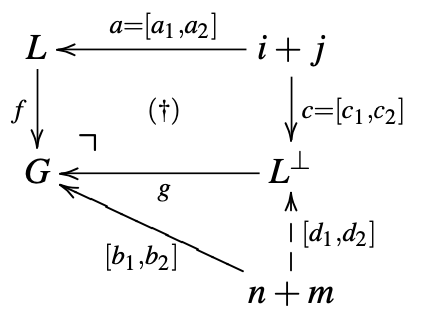
\includegraphics[width=0.4\linewidth]{figures/combinatorial_semantics/boundary_complement.png}
% \end{figure}

% https://q.uiver.app/#q=WzAsNSxbMCwwLCJMIl0sWzIsMCwiaStqIl0sWzAsMiwiR157XFx1cmNvcm5lcn0iXSxbMiw0LCJuK20iXSxbMiwyLCJMXntcXGJvdH0iXSxbMyw0LCJbZF8xLGRfMl0iLDJdLFszLDIsIltiXzEsYl8yXSJdLFswLDIsImYiLDJdLFsxLDAsImEgPSBbYV8xLGFfMl0iLDJdLFsxLDQsImMgPSBbY18xLGNfMl0iXSxbNCwyLCJnIl1d
\[\begin{tikzcd}
	\mathcal L && {i+j} \\
	\\
	{\mathcal G^{\urcorner}} && {\mathcal{L}^{\bot}} \\
	\\
	&& {n+m}
	\arrow["{[d_1,d_2]}"', from=5-3, to=3-3]
	\arrow["{[b_1,b_2]}", from=5-3, to=3-1]
	\arrow["f"', from=1-1, to=3-1]
	\arrow["{[a_1,a_2]}"', from=1-3, to=1-1]
	\arrow["{[c_1,c_2]}", from=1-3, to=3-3]
	\arrow["g", from=3-3, to=3-1]
\end{tikzcd}\]
is called a boundary complement if $[c_1, c_2]$ is mono and there exist $d_1 : n \to \mathcal{L}^{\bot}$ and $d_2 : m \to \mathcal{L}^{\bot}$ making the above triangle commute and such that
\[
    n + j \xrightarrow{[d_1,c_2]} \mathcal{L}^{\bot} \xleftarrow{[d_2,c_1]} m + i
\]
is a monogamous cospan. 
\end{definition}
%\begin{remark}
%    Note how the requirement for $i \xrightarrow{} L \xleftarrow{} j$ and $n \xrightarrow{} G \xleftarrow{} m$ being monogamous, i.e. morphisms in $\MdaCospans$, is a part of the above definition.
%\end{remark}
Intuitively,  requiring boundary complements ensures that inputs are glued exclusively to outputs and vice-versa in the two pushout squares.

\begin{definition}[Convex match]
We call a subgraph $\mathcal{H}$ of a hypergraph $\mathcal{G}$ a \emph{convex subgraph} if for all $v_i, v_j \in V_{\mathcal{H}}$ every path from $v_i$ to $v_j$ is also in $\mathcal{H}$.
We call a match $m : \mathcal L \to \mathcal G$ a \emph{convex match} if it is mono and its image is a convex subgraph of $\mathcal G$. 
   
\end{definition}

\begin{definition}[Convex DPOI rewriting]
Let $\mathfrak{R}$ be a set of DPOI rewrite rules. 
Then, given $\mathcal G \xleftarrow{} n+m$ and $\mathcal H \xleftarrow{} n + m$ in $\catname{Hyp(\Sigma)}$, $\mathcal G$ rewrites convexly into $\mathcal H$ with interface $n + m$ --- notation $(\mathcal G \xleftarrow{} n + m ) \Rrightarrow_{\mathfrak{R}}  (\mathcal H \xleftarrow{} n + m )$ --- if there exist rule $\mathcal L \xleftarrow{} i + j \xrightarrow{} \mathcal R$ in $\mathcal{R}$ and object $C$ and cospan arrows $i+j \xrightarrow{} \mathcal C \xleftarrow{} n+m$ such that the DPOI diagram of Definition \ref{def:dpoi} commutes and its marked squares are pushouts 
and the following conditions hold
\begin{itemize}
    \item $m : L \to \mathcal G$ is a convex match;
    \item $i + j \to \mathcal C \to \mathcal G$ is a boundary complement in the leftmost pushout.
\end{itemize}
\end{definition}
%By requiring convex matching and boundary complements we ensure that the original cospans above are monogamous, e.g., $n \xrightarrow{} G \xleftarrow{} m$.

CHRIS: WANT TO STATE THE CORRESPONDENCE THEOREM WITH SMTS HERE? NEED TO DEFINE $\lceil-\rceil$ AND INTERPRETATION? Hmm
\begin{theorem}[Theorem 35~\cite{Frobenius2}]
For any $f,g \in \mathbf{SMT}(\Sigma, \mathcal{E})$,  we have that 
\[
	f = g \iff \llangle \lceil f \rceil \rrangle \Rrightarrow^*_{\mathfrak{R}} \llangle \lceil g \rceil \rrangle~, 
\]
where $\mathfrak{R} = \llangle \lceil \mathcal{E} \rceil \rrangle$ and $ \Rrightarrow^*_{\mathfrak{R}}$ denotes the existence of a sequence of convex rewrites. 
\end{theorem}
\section{E-Hypergraphs}

WHAT DOES (3) FOR CONSISTENCY MEAN? 
In this section,  we follow analogous steps to those used to achieve a combinatorial representation of $\textbf{PROP}(\Sigma)$ by $\mathbf{MHypI}(\Sigma)$,  but in our semilattice enriched setting.  First we define an \textit{e-hypergraph},  which supports a hierarchical notion of "e-box" with distinct components. Then,  we extend this notion with interfaces via a generalization of the cospan construction.  Finally,  we restrict the morphisms under consideration to those satisfying the MDA condition,  as in the previous section.  An example diagram representing our e-hypergraphs with interfaces can be found in Figure \ref{fig:A+B}.

Note that here,  and in the rest of the paper,  we will restrict to dealing with signatures $\Sigma$ containing only morphisms $f: n \to m$ where either $n$ or $m$ are non-zero.  This is a restriction we make in order to avoid complications to the technical development of DPOI rewriting for e-hypergraphs given in the subsequent section,  and we explain it further there. 

In the following,  we elide the obvious injections of $V$ and $E$ into $V+E$. 
\begin{definition}[Category of E-hypergraphs]
\label{def:e-homo}    
An \emph{e-hypergraph $\mathcal{G}$ over a signature $\Sigma$} is a tuple $(V,E,s,t,l,<,\consistency)$,  where $(V,E,s,t)$ is an unlabelled hypergraph;  $l :E \to \Sigma + 1$ is a labelling function modified to include an extra value $\bot$ in its codomain; $<$ is a strict partial order on $V + E$ called the \textit{child relation}; and an equivalence relation $\consistency$ on $V + E$ called the \textit{consistency relation}.  We define the following additional notation.  For $x \in V + E$,  the set of \emph{parents} and \emph{children} of $x$,  respectively: 
\[
	[x) = \{x' ~|~ x' <_c x\; \} \qquad (x] = \{x' ~|~  x <_{c} x'\}
\]
We will denote the unique immediate parent $e$ of $x$ by writing $e <^{\mu} x$.
We call edges $e$ such that $l(e) = \bot$ \textit{hierarchical},  and edges $e$ and nodes $v$ such that $[e) = \varnothing$ and $[v) = \varnothing$ \emph{top-level}.
We require that the child relation satisfies the following conditions:
\begin{enumerate}
	\item each parent set contains exclusively hierarchical edges;
	\item Each $x$ has at most one immediate parent;
	\item if $v \in s(e)$ then $e' <^{\mu} e$ iff $e' <^{\mu} v$.
\end{enumerate}
The consistency equivalence relation must satisfy the following conditions:
    \begin{enumerate}
        \label{def:consistency_properties}
        \item If $v \in s(e)$ or $v \in t(e)$ then $v \consistency e$;
        \item The relation is defined only for edges $x$ which are not top-level.
    \end{enumerate}

A homomorphism $\phi: \mathcal{F} \to \mathcal{G}$ of e-hypergraphs $\mathcal{F},\mathcal{G}$ is a pair of functions $\phi_V : V_{\mathcal{F}} \to V_{\mathcal{G}}, \phi_E : E_{\mathcal{F}} \to E_{\mathcal{G}}$ such that
\begin{enumerate}
    \item $\phi$ is a hypergraph homomorphism
    \item for $v \in V_{\mathcal{F}}$,  if $[v)$ is not empty then 
	\[
        \phi_{E}(<_{\mathcal{F}}^{\mu}(v)) = <_{\mathcal{G}}^{\mu}(\phi_{V}(v))
        \] 
        and for $e \in E_{\mathcal{F}}$,  if $[e)$ is not empty then 
        \[
        \phi_{E}(<_{\mathcal{F}}^{\mu}(e)) = <_{\mathcal{G}}^{\mu}(\phi_{E}(e))  
        \] 
    % \item
    % $x_1 \#_{\mathcal{F}} x_2$ iff $\phi(x_1) \#_{\mathcal{G}} \phi(x_2)$, where $x_1, x_2 \in \mathcal{F}$
        \item for all $x_1, x_2 \in \mathcal{F}$,  $x_1 \consistency_{\mathcal{F}} x_2$ implies $\phi(x_1) \consistency_{\mathcal{G}} \phi(x_2)$. 
%    Or, written functionally, when $x \in E_{\mathcal{F}}$
%    \[
%        \langle \phi_{V};i_{V_{\mathcal{G}}}, \phi_{E};i_{E_{\mathcal{G}}} \rangle^{*}(\consistency_{\mathcal{F}}^{\mu}(i_{E_{\mathcal{F}}}(x)))
%        \subseteq
%        \consistency_{\mathcal{G}}^{\mu}(\phi_{E};i_{E_{\mathcal{G}}}(x))
%    \]
%    , where $\phi_{V};i_{V_{\mathcal{G}}} : V_{\mathcal{F}} \to V_{\mathcal{G}} + E_{\mathcal{G}}$%, and similarly for $\phi_{E};i_{E_\mathcal{G}}$ so that $\langle \phi_{V};i_{V_{\mathcal{G}}}, \phi_{E};i_{E_{\mathcal{G}}} \rangle : V_{\mathcal{F}} + E_{\mathcal{F}} \to  V_{\mathcal{G}} + E_{\mathcal{G}}$.
%    And, when $x \in V_{\mathcal{F}}$
%    \[
%        \langle \phi_{V};i_{V_{\mathcal{G}}}, \phi_{E};i_{E_{\mathcal{G}}} \rangle^{*}(\consistency_{\mathcal{F}}^{\mu}(i_{V_{\mathcal{F}}}(x)))
%        \subseteq
%        \consistency_{\mathcal{G}}^{\mu}(\phi_{V};i_{V_{\mathcal{G}}}(x))
%    \]
    % Or, on per-component basis, if $i_{E_{\mathcal{F}}}(x_1) \in \hashtag_{\mathcal{F}}(i_{E_{\mathcal{F}}}(x_2))$ then $i_{E_{\mathcal{G}}}(\phi_{E}(x_1)) \in \hashtag_{\mathcal{G}}(i_{E_{\mathcal{G}}}(\phi_{E}(x_2)))$ and similarly for other types of $x_1,x_2$.
\end{enumerate}
If we further have that if $[x_1) = \varnothing$ then $[\phi(x_1)) = \varnothing$ we call the homomorphism \textit{strict}.
The \emph{category of e-hypergraphs},  denoted  $\catname{EHyp(\Sigma)}$,  has e-hypergraphs as objects and e-hypergraph homomorphisms as arrows.  
\end{definition}
Intuitively,  the child relation equips the hypergraph with a hierarchical structure: certain edges,  labelled with $\bot$,  are meant to interpret the dashed e-boxes of our string diagrams.  
These edges can be designated as "parents" to sub-hypergraphs,  which interpret the various components of the e-boxes.  These components are distinguished by the consistency relation, which partitions the sub-hypergraph below the hierarchical edge.  
Technically,  condition $(3)$ on the child relations says that $<^{\mu}$ respects connectivity of edges and vertices,  and similarly for conditions $(1)$ of the consistency relation. 
The conditions on homomorphisms require to preserve immediate parents and the conflict relation.  

The category of e-hypergraphs has coproducts,  given by the disjoint union of e-hypergraphs,  and an initial object given by the empty e-hypergraph.  A concrete description of the pushout of two morphisms in this category is given in the appendix.  Generally,  the pushout of two e-hypergraph homomorphisms need not exist,  but we prove that it does when certain technical conditions are satisfied,  including that the two morphisms involved are monos and their shared domain is a discrete hypergraph.  

\begin{remark}
When we wish to consider $\phi(\mathcal{F}) \subseteq \mathcal{G}$ as an e-hypergraph in its own right,  we assign $\bot$ to be the immediate parent of all $x$ whose immediate parent is in $\mathcal{G}$ is outside $\phi(\mathcal{F})$.
\end{remark}

When modelling our enriched string diagrams using e-hypergraphs,  we require to keep track of more than simply the ultimate external inputs and outputs of the diagram: each internal e-box has its own inputs and outputs,  which we must also keep track of.  Thus,  we introduce an \textit{extended} cospan construction.  Since the $\catname{EHyp(\Sigma)}$ does not have pushouts in general,  we skip straight to considering a category of extened cospans of discrete e-hypergraphs (\textit{i.e.},  discrete hypergraphs considered as e-hypergraphs in the obvious way),  for which pushouts do exist. 
\begin{definition}[Category of e-hypergraphs with interfaces]
    We will build the category of \textit{e-hypergraphs with interfaces},  denoted $\Ecospans$ as follows.  Its objects are discrete e-hypergraphs,  and the set of morphisms $\Ecospans(n,m)$ are isomorphism classes of \textit{extended cospans},  which are defined as follows:  
    \[
    n \xrightarrow{f_{ext}} n' \xrightarrow{f_{int}} \mathcal{G} \xleftarrow{g_{int}} m' \xleftarrow{g_{ext}} m
    \]
    where $\mathcal{G}$ is an e-hypergraph,  and $n, n', m, m'$ are discrete e-hypergraphs,  $f_{ext},f_{int},g_{ext},g_{int}$ are monomorphisms in $\catname{EHyp(\Sigma)}$,  and the image of $f_{ext};f_{int}$ and of $g_{ext};g_{int}$ consist exclusively of top-level vertices.  

This justifies calling $n$  \textit{external input interfaces} and $n'$ \textit{internal input (output) interfaces}.  We call $n' \setminus f_{ext}(n)$  the \textit{strictly internal input interfaces}.  We do analogously for the \emph{output interfaces},  with respect to $m$,  $m'$ and $m' \setminus g_{ext}(m)$.  
We will sometimes confuse $f_{ext}$ with $f_{ext};f_{int}$ when it is clear from context,  and we will sometimes confuse $n, n', m$ and $m'$ with their images in $\mathcal{G}$. 
Given an edge $e \in E_\mathcal{G}$ such that $l(e) = \bot$,  we call the \textit{inputs of $e$} the intersection of the strictly internal input interface of $\mathcal{G}$ with the immediate successors of $e$,  and analogously for the \emph{outputs of $e$}. 
    
    Two cospans are isomorphic if there exist isomorphisms $\alpha$, $\beta$ and $\gamma$ making the following diagram commute.
    \[
    \scalebox{0.75}{
        \tikzfig{combinatorial_semantics/isomorphic_e_cospans}
    }
    \]
Composition of two morphisms $f : X_{ext} \to Y_{ext}$ and $g : Y_{ext} \to Z_{ext}$ is computed in two stages
First, $\mathcal{F} +_{f_{ext}, g_{ext}} \mathcal{G}$ is computed,  as shown below. 

% https://q.uiver.app/#q=WzAsMTAsWzAsMCwiZXh0KFgpIl0sWzEsMSwiWCJdLFsyLDIsIkEiXSxbMywwLCJZIl0sWzQsMCwiZXh0KFkpIl0sWzUsMCwiWSciXSxbNiwyLCJCIl0sWzcsMSwiWiJdLFs4LDAsImV4dChaKSJdLFs0LDMsIl57XFx1bGNvcm5lcn1BK197Zl97ZXh0fTtmLGdfe2V4dH07Z31CIl0sWzAsMV0sWzEsMl0sWzMsMiwiZiJdLFs0LDMsImZfe2V4dH0iXSxbNCw1LCJnX3tleHR9IiwyXSxbNSw2LCJnIiwyXSxbNyw2XSxbOCw3XSxbMiw5XSxbNiw5XV0=

\[
\scalebox{0.9}
{\tikzfig{combinatorial_semantics/pushout_e_cospans}}
\]
Then, new feet for $\mathcal{H} = A +_{f_{ext};f,g_{ext};g} B$ are computed as below
\[
X_{ext} \xrightarrow{a_{ext};\iota_1} X \uplus (Y' \setminus Y_{ext}) \xrightarrow{h} \mathcal{H} \xleftarrow{k} Z \uplus (Y \setminus Y_{ext}) \xleftarrow{g_{ext};\iota_1} Z_{ext}
\]
where
\[
    h = \langle a;p_1, g|_{Y' \setminus Y_{ext}};p_2 \rangle
\]
 
\[
    k = \langle b;p_2, f|_{Y \setminus Y_{ext}};p_1 \rangle
\]
% \[
% \begin{tikzcd}
% Y_{ext} \arrow[d] & 0 \arrow[l] \arrow[d]    \\
% Y'          & Y' \setminus Y_{ext} \arrow[l]
% \end{tikzcd}
% \]
% and then the disjoint union is just a coproduct. 
The identity of composition is given by the obvious extended cospan of identities. 
$\Ecospans$ inherits a symmetric monoidal structure from the coproduct (and initial object) structure of $\catname{EHyp_{\Sigma}}$,  analogously to Definition~\ref{def:cspd}.  
\end{definition}
CHRIS: UPDATE DIAGRAMS TO USE MY NEW NOTATION,  TAKE LESS VERTICAL SPACE.  FIND CLEANER WAY TO WRITE NEW FEET.  USE $\iota$ FOR INJECTIONS,  WHAT IS $\langle \rangle$? Include example e-hypergraph-with-interfaces vs strings here? 

As in the standard cospan construction,  it is necessary to consider isomorphism classes of cospans since composition (defined by pushout) is associative only up-to isomorphism (since pushouts are unique only up-to isomorphism). 
% https://q.uiver.app/#q=WzAsNSxbMCwwLCJYICsgWSJdLFsyLDAsIlggKyBZIl0sWzQsMCwiWSArIFgiXSxbNiwwLCJZICsgWCJdLFs4LDAsIlkgKyBYIl0sWzAsMSwiaWRfWCArIGlkX1kiXSxbMSwyLCJcXHNpZ21hX3tYLFl9Il0sWzQsMywiaWRfWSArIGlkX1giLDJdLFszLDIsImlkX1kgKyBpZF9YIiwyXV0=



\begin{definition}[Category of well-typed MDA e-hypergraphs with interfaces]
We call an extended cospan in $\Ecospans$,  as below,   \textit{monogamous directed acyclic (MDA)} if
\[
n \xrightarrow{f_{ext}} n' \xrightarrow{f_{int}} \mathcal{G} \xleftarrow{g_{int}} m' \xleftarrow{g_{ext}} m
\]
\begin{enumerate}
        \item underlying hypergraph of $\mathcal{G}$ is directed acyclic; 
        \item $f_{ext}$, $f_{int}$, $g_{ext}$ and $g_{int}$ are monomorphisms; 
        \item The in-degree and out-degree of every vertex is at most 1; 
        \item Vertices with in-degree $0$ are precisely the image of $f_{int}$; 
        \item Vertices with out-degree $0$ are precisely the image of $g_{int}$; 
        \item Vertices in the strictly internal interface are not top-level. 
        % the item below is not assumed by the definition of a cospan of e-hypergraphs
        % \item $[v) = \varnothing$ for all $v$ in the image of $f_{ext};f$, and for all $v$ in the image of $g_{ext};g$. 
\end{enumerate}
\label{def:monogamy_ehyp} 

Further,  consider the sets of input and output vertices,  $I$ and $O$ respectively,  of a hierarchical edge $e$ of an e-hypergraph $\mathcal{G}$. 
The consistency relation of $\mathcal{G}$ partitions $I$ and $O$.  
We call $e$ \emph{well-typed} if the size of each partition of $I$ is $|s(e)|$ and the size of each partition of $O$ is $|t(e)|$.
We will call an MDA-extended-cospan in $\MdaEcospans$ \emph{well-typed} if all hierarchical edges in its apex are well-typed.

We denote by $\MdaEcospans$ the subcategory of $\Ecospans$ consisting of well-typed MDA-extended-cospans. 
\end{definition}
CHRIS: COULD PUT CONDITION (5) IN THE PLAIN DEFINITION OF EXTENDED COSPANS? WE ALREADY ASK FOR EXTERNAL INTERFACES TO BE TOP-LEVEL.  ALSO,  (2) IS ALREADY COVERED IN THAT DEFINITION. 

Unlike in the previous section,  in order to give an equivalence with $\textbf{PROP}^+(\Sigma)$,  we must first develop the theory of DPOI rewriting for e-hypergraphs.  This is beacuse the equations for semilattice enrichment are not intended to be subsumed by the e-hypergraph representation.  Instead,  we will treat them via rewriting,  as we do with equations of the signature.  This is because the semilattice equations involve (un)sharing,  and so we wish to maintain distinct e-hypergraphs expressing more or less shared representations of morphisms. 

\section{DPOI-Rewriting for E-Hypergraphs}

CHRIS: REMARK THAT WE CANNOT DEAL WITH SIGNATURES WITH $f:0 \to 0$ MORPHISMS, AND WHY!
As extended cospans have a more general notion of interface we need to make some adjustments to DPOI rewriting.
The main issue is that internal interfaces may not be preserved during rewriting, for example, if the right-hand side of the rewrite rule has more hierarchy than the left-hand side: it affects both the eventual e-hypergraph and the possible pushout complement.

% The input interface on the left-hand side of the rule is $\{1, 2\}$, while the input interface on the right-hand side of the rule is $\{1,2,5,6,7,8\}$.
% Note that the outermost interfaces are preserved.

% Another concern is when we delete the occurrence of the left-hand side of a rewrite rule from an e-hypergraph we also modify this e-hypergraph's interfaces.
% Consider a hypothetical DPO square below in Figure~\ref{fig:interface_change_example} where long arrows denote matching between carriers of cospans.

% The first row of the diagram shows the span for a rewrite rule of $\langle f + g, f \rangle$ which is like a projection rule.
% Note once again the difference between the interfaces of the left-hand and right-hand sides of the rewrite rule.
% The entry in the middle of the span depicts the outermost interfaces which are preserved.
% The second row depicts the e-hypergraph to be rewritten on the left and the result of the rewrite on the right.
% The result is obtained by first deleting the image of the left-hand side of the rewrite rule from the initial e-hypergraph (depicted in the middle) and then gluing the right-hand side of the rewrite rule into it. 
% Note that the interfaces of the initial e-hypergraph and the residual e-hypergraph are different. 
% Here, the outermost and the whole interfaces for the eventual e-hypergraph coincide, but if the nested-ness of the initial e-hypergraph was more intense the result could have inner interfaces as well as we would remove the interfaces of the inner edges when deleting the image of the left-hand side part of the rule from the initial e-hypergraph.

To account for such changes in the interfaces we put some additional constraints on DPOI rewriting for the case of $\catname{EHyp_{\Sigma}}$.
Consider a DPOI diagram with extra constraints below which encodes
the notion that e-hypergraph $G$ rewrites into $H$ with external interfaces $n_{ext}+m_{ext}$.
Note the new interfaces and how we use the same trick to go from cospan $n_{ext} \xrightarrow{} g_i \xrightarrow{} G \xleftarrow{} g_o \xleftarrow{} m_{ext}$ to $G \xleftarrow{} g_{i} + g_{o} \xleftarrow{} n_{ext} + m_{ext}$.
The original DPO square is depicted in blue.
% \[\begin{tikzcd}
% 	&&&& {i + j} \\
% 	{l_i+l_o} && L &&&& R && {r_i+r_o} \\
% 	\\
% 	{g_i+g_o} && {G^{\urcorner}} && C && {^{\ulcorner}H} && {h_i+h_o} \\
% 	\\
% 	&&&& {n+m}
% 	\arrow[color={rgb,255:red,214;green,92;blue,92}, from=1-5, to=2-3]
% 	\arrow[color={rgb,255:red,214;green,92;blue,92}, from=1-5, to=2-7]
% 	\arrow["m", color={rgb,255:red,214;green,92;blue,92}, from=2-3, to=4-3]
% 	\arrow["{[i_c,j_c]}", color={rgb,255:red,214;green,92;blue,92}, from=1-5, to=4-5]
% 	\arrow[color={rgb,255:red,214;green,92;blue,92}, from=2-7, to=4-7]
% 	\arrow["{[n_c,m_c]}"', color={rgb,255:red,214;green,92;blue,92}, from=6-5, to=4-5]
% 	\arrow[color={rgb,255:red,214;green,92;blue,92}, from=4-5, to=4-7]
% 	\arrow[color={rgb,255:red,214;green,92;blue,92}, from=4-5, to=4-3]
% 	\arrow[color={rgb,255:red,214;green,92;blue,92}, from=6-5, to=4-3]
% 	\arrow[color={rgb,255:red,214;green,92;blue,92}, from=6-5, to=4-7]
% 	\arrow[from=2-1, to=2-3]
% 	\arrow["{[f_i,f_o]}", from=2-1, to=4-1]
% 	\arrow[from=4-1, to=4-3]
% 	\arrow[from=2-9, to=2-7]
% 	\arrow[from=4-9, to=4-7]
% 	\arrow["{[h_i,h_o]}"{description}, from=2-9, to=4-9]
% 	\arrow[from=6-5, to=4-9]
% 	\arrow[from=6-5, to=4-1]
% 	\arrow["{[i_l,j_l]}"{description}, from=1-5, to=2-1]
% 	\arrow["{[i_r,j_r]}"{description}, from=1-5, to=2-9]
% \end{tikzcd}\]


% https://q.uiver.app/#q=WzAsMTEsWzIsMCwiTCJdLFs0LDAsInhfe2V4dH0gKyB5X3tleHR9Il0sWzIsMiwiR157XFx1cmNvcm5lcn0iXSxbNCwyLCJDIl0sWzQsNCwibl97ZXh0fSttX3tleHR9Il0sWzAsMCwibF9pK2xfbyJdLFswLDIsImdfaStnX28iXSxbNiwwLCJSIl0sWzYsMiwiXntcXHVsY29ybmVyfUgiXSxbOCwyLCJoX2kraF9vIl0sWzgsMCwicl9pK3JfbyJdLFsxLDAsIiIsMCx7ImNvbG91ciI6WzAsNjAsNjBdfV0sWzAsMiwibSIsMCx7ImNvbG91ciI6WzAsNjAsNjBdfSxbMCw2MCw2MCwxXV0sWzEsMywiW2lfYyxqX2NdIiwwLHsiY29sb3VyIjpbMCw2MCw2MF19LFswLDYwLDYwLDFdXSxbNCwzLCJbbl9jLG1fY10iLDIseyJjb2xvdXIiOlswLDYwLDYwXX0sWzAsNjAsNjAsMV1dLFszLDIsIiIsMix7ImNvbG91ciI6WzAsNjAsNjBdfV0sWzQsMiwiIiwyLHsiY29sb3VyIjpbMCw2MCw2MF19XSxbNSwwXSxbNiwyXSxbNCw4LCIiLDAseyJjb2xvdXIiOlswLDYwLDYwXX1dLFszLDgsIiIsMCx7ImNvbG91ciI6WzAsNjAsNjBdfV0sWzcsOCwiIiwyLHsiY29sb3VyIjpbMCw2MCw2MF19XSxbMSw3LCIiLDIseyJjb2xvdXIiOlswLDYwLDYwXX1dLFsxMCw3XSxbOSw4XV0=
\[
 \scalebox{0.75}{
    \tikzfig{combinatorial_semantics/DPOI_square_coloured}
 }
\]

% The parts of the original DPOI square is shown in blue.
% For example, the left-hand side $L$ of a rewrite rule
%  $\langle L, R \rangle$ which originally was some cospan
%  $i \xrightarrow{} L \xleftarrow{} j$ in $\MdaCospans$ 
%  now is a cospan
%  $x_{ext} \xrightarrow{} l_i \to L \xleftarrow{} l_o \xleftarrow{} y_{ext}$
% from $\WellTypedMdaEcospans$ where $l_i, l_o$ are whole input and output interfaces respectively.
% The top half of this diagram says that the outermost interfaces
%  should coincide for $L$ and $R$.
% The bottom half puts the same restrictions on $G$ and $H$.
% For the pushout to exist we impose our assumptions~\ref{pushout:assumptions} on the correspoding arrow.


We then also adjust the definition of a boundary complement.

\begin{definition}[Boundary complement in $\WellTypedMdaEcospans$]
\label{def:boundary_new}

% https://q.uiver.app/#q=WzAsNyxbMiwwLCJMIl0sWzQsMCwieF97ZXh0fSArIHlfe2V4dH0iXSxbMiwyLCJHXntcXHVyY29ybmVyfSJdLFs0LDIsIkMiXSxbNCw0LCJuX3tleHR9K21fe2V4dH0iXSxbMCwwLCJsX2krbF9vIl0sWzAsMiwiZ19pK2dfbyJdLFsxLDAsIiIsMCx7ImNvbG91ciI6WzAsNjAsNjBdfV0sWzAsMiwibSIsMCx7ImNvbG91ciI6WzAsNjAsNjBdfSxbMCw2MCw2MCwxXV0sWzEsMywiW2lfYyxqX2NdIiwwLHsiY29sb3VyIjpbMCw2MCw2MF19LFswLDYwLDYwLDFdXSxbNCwzLCJbbl9jLG1fY10iLDIseyJjb2xvdXIiOlswLDYwLDYwXX0sWzAsNjAsNjAsMV1dLFszLDIsIiIsMix7ImNvbG91ciI6WzAsNjAsNjBdfV0sWzQsMiwiIiwyLHsiY29sb3VyIjpbMCw2MCw2MF19XSxbNSwwXSxbNiwyXV0=

For monogamous extended cospans $x_{ext} \xrightarrow{} l_{i} L \xleftarrow{} l_{o} \xleftarrow{} y_{ext}$ and $n_{ext} \xrightarrow{} g_{i} \xrightarrow{} G \xleftarrow{} g_{o} \xleftarrow{} m_{ext}$ and mono $f : L \to G$, a pushout complement $x_{ext} + y_{ext} \to C \to G^{\urcorner}$ as depicted below
\[
\scalebox{0.75}{

    \tikzfig{combinatorial_semantics/DPOI_pushout_complement}
}
\]


is a \textit{boundary} complement if $[i_c, i_j]$ is mono 
 and there exist $n_c : n_{ext} \to C$ and $m_c : m_{ext} \to C$ 
 making the above triangle commute and such that
there exists a \textit{not necessarily well-typed} mda-cospan

\[
n_{ext} \xrightarrow{} c_i + y_{ext} \xrightarrow{} C \xleftarrow{} c_o + x_{ext} \xleftarrow{} m_{ext}
\]

where $c_i$ and $c_o$ are computed as
 $c_i = g_i \setminus (l_i \setminus x_{ext})$ and
 $c_o = g_o \setminus (l_o \setminus y_{ext})$.

 ALEKSEI: ARE MORPHISMS $c_i + y_{ext} \to C$ AND THE SYMMETRIC ONE OBVIOUS?
\end{definition}
%
%\begin{figure}
%    \centering
%    \[
%    \scalebox{0.5}{\tikzfig{combinatorial_semantics/interfaces_change_example}}\]
%    \caption{Hypothetical DPO square for $\catname{MACsp_{D}(EHyp_{\Sigma})}$}
%    \label{fig:interface_change_example}
%\end{figure}

% The second point above means that when cutting the mono-occurrence of $L$ out from $G$ we also need to remove the inner interfaces of $L$ from the whole interface of $G$. \question{According to the pushout squares above, $c_i$ is constructed by removing from $g_i$ everything from $l_i$ which does not have a pre-image in $i$, i.e., everything except the outermost interfaces (same holds for $c_o$)}

\begin{remark}
Note that cospan $n_{ext} \xrightarrow{} c_i + y_{ext} \xrightarrow{} C \xleftarrow{} c_o + x_{ext} \xleftarrow{} m_{ext}$ is not necessarily well-typed.
The cospan's input internal interface may contain nodes that previously were a part of the output internal interface and similarly for output internal interface.
\end{remark}

\begin{remark}
    The uniqueness and existence properties of such pushout complement are discussed in the appendix (Proposition~\ref{prop:boundary_complement} and Proposition~\ref{prop:complement_existence}).
\end{remark}


% \begin{proposition}[Proposition~\ref{prop:boundary_complement} restatement]
%     The boundary complement in~\ref{def:boundary_new} when exists is unique.
% \end{proposition}

\begin{definition}[Down-closed subgraph]
    We call a subgraph $\mathcal{H}$ of an e-hypergraph $\mathcal{G}$ \emph{down-closed} if for all $e \in E_{\mathcal{H}}$,   every element of $(e]$ is also in $\mathcal{H}$.
\end{definition}    

\begin{definition}[Convex down-closed match] 
    We call $m : L \to G$ in $\catname{EHyp_{\Sigma}}$ a convex down-closed match if
    
    \begin{enumerate}
        \item $m$ is monomorphism
        \item $m(L)$ is a convex down-closed subgraph of $G$
    \end{enumerate}
\end{definition}
\

\begin{definition}[Rewriting in $\WellTypedMdaEcospans$]
    Given $G \xleftarrow{} g_i + g_o \xleftarrow{} n_{ext} + m_{ext}$ 
    and $H \xleftarrow{} h_i + h_o \xleftarrow{} n_{ext} + m_{ext}$ in $\Ecospans$ with the outermost interfaces $n_{ext} + m_{ext}$, $G$ rewrites convexly into $H$ with the outermost interface $n_{ext} + m_{ext}$ --- notation $( G \xleftarrow{} n_{ext} + m_{ext} ) \Rrightarrow_{\mathcal{R}}^{+} (E \xleftarrow{} n_{ext} + m_{ext} )$ --- if there exists a rule $L \xleftarrow{} l_i + l_o \xleftarrow{} x_{ext} + y_{ext} \xrightarrow{} r_i + r_o \xrightarrow{} R$ with the outermost interfaces $x_{ext} + y_{ext}$ in the set of rewrite rules $\mathcal{R}$ and object $C$ and cospan arrows $x_{ext} + y_{ext} \xrightarrow{} C \xleftarrow{} n_{ext} + m_{ext}$ such that the diagram below commutes and its marked squares are pushouts

% https://q.uiver.app/#q=WzAsMTEsWzIsMCwiTCJdLFs0LDAsInhfe2V4dH0gKyB5X3tleHR9Il0sWzIsMiwiR157XFx1cmNvcm5lcn0iXSxbNCwyLCJDIl0sWzQsNCwibl97ZXh0fSttX3tleHR9Il0sWzAsMCwibF9pK2xfbyJdLFswLDIsImdfaStnX28iXSxbNiwwLCJSIl0sWzYsMiwiXntcXHVsY29ybmVyfUgiXSxbOCwyLCJoX2kraF9vIl0sWzgsMCwicl9pK3JfbyJdLFsxLDAsIiIsMCx7ImNvbG91ciI6WzAsNjAsNjBdfV0sWzAsMiwibSIsMCx7ImNvbG91ciI6WzAsNjAsNjBdfSxbMCw2MCw2MCwxXV0sWzEsMywiW2lfYyxqX2NdIiwwLHsiY29sb3VyIjpbMCw2MCw2MF19LFswLDYwLDYwLDFdXSxbNCwzLCJbbl9jLG1fY10iLDIseyJjb2xvdXIiOlswLDYwLDYwXX0sWzAsNjAsNjAsMV1dLFszLDIsIiIsMix7ImNvbG91ciI6WzAsNjAsNjBdfV0sWzQsMiwiIiwyLHsiY29sb3VyIjpbMCw2MCw2MF19XSxbNSwwXSxbNiwyXSxbNCw4LCIiLDAseyJjb2xvdXIiOlswLDYwLDYwXX1dLFszLDgsIiIsMCx7ImNvbG91ciI6WzAsNjAsNjBdfV0sWzcsOCwiIiwyLHsiY29sb3VyIjpbMCw2MCw2MF19XSxbMSw3LCIiLDIseyJjb2xvdXIiOlswLDYwLDYwXX1dLFsxMCw3XSxbOSw4XV0=
\[\scalebox{0.75}{
    \tikzfig{combinatorial_semantics/DPOI_square}
    }
\]
    and the following conditions hold

    \begin{enumerate}
        \label{dpoi:assumptions}
        \item $m : L \to G$ is a convex down-closed match;
        \item $x_{ext} + y_{ext} \to C \to G$ is a boundary complement in the leftmost pushout.
    \end{enumerate}
\end{definition}


The internal interfaces of the resulting e-hypergraph $H$ from the cospan
 $n_{ext} \xrightarrow{} h_i \xrightarrow{} H \xleftarrow{} h_o \xleftarrow{} m_{ext}$
 are constructed as $h_i = (r_i \setminus x_{ext}) + c_i$ 
 and
 $h_o = (r_o \setminus y_{ext}) + c_o$.
 $h_i \to H$ is defined as a copairing of 
 $f_1 : r_i \setminus x_{ext} \to R \to H$ 
 and 
 $f_2 : c_i \to C \to H$. 
Since both $f_1$ and $f_2$ are mono, their copairing is also a mono. 
Similarly for $h_o$.

We then say that an mda-cospan 
\[
    n_{ext} \xrightarrow{a_1} g_{i} \xrightarrow{a_2} G \xleftarrow{b_2} g_{o} \xleftarrow{b_1} m_{ext}
\]
rewrites convexly into another mda-cospan

\[
    n_{ext} \xrightarrow{a_1} h_{i} \xrightarrow{a_2} H \xleftarrow{b_2} h_{o} \xleftarrow{b_1} m_{ext}
\]

under a rewrite rule 
\[
    \langle x_{ext} \xrightarrow{a_1} l_{i} \xrightarrow{a_2} L \xleftarrow{b_2} l_{o} \xleftarrow{b_1} y_{ext}, 
    x_{ext} \xrightarrow{a_1} r_{i} \xrightarrow{a_2} R \xleftarrow{b_2} r_{o} \xleftarrow{b_1} y_{ext} \rangle
\]

if 
\begin{align*}    
    G \xleftarrow{\langle a_2,b_2 \rangle} g_i + g_{o}& \xleftarrow{\langle a_1, b_1 \rangle} n_{ext} + m_{ext} \\ &\Rrightarrow^{+}\\ H \xleftarrow{\langle a_2,b_2 \rangle} h_i + h_{o}& \xleftarrow{\langle a_1, b_1 \rangle} n_{ext} + m_{ext}
\end{align*}

under a rewrite rule
\[
    \langle l_{i} + l_{o} \xrightarrow{\langle a_2, b_2 \rangle} L \xleftarrow{\langle a_1, b_1 \rangle} x_{ext} + y_{ext},
    r_{i} + r_{o} \xrightarrow{\langle a_2, b_2 \rangle} R \xleftarrow{\langle a_1, b_1 \rangle} x_{ext} + y_{ext} 
    \rangle
\]

\begin{proposition}
$n_{ext} \xrightarrow{n_h} h_i \xrightarrow{f} H \xleftarrow{g} h_o \xleftarrow{m_h} m_{ext}$ is a well-typed mda-cospan.
\end{proposition}

\section{Soundness and Completeness}\label{sec:soundness-and-completeness}

% \update{below definition depends on whether we require the homomorphism to reflect the conflicts}



\begin{figure}
    \[
    \scalebox{0.6}{
    \tikzfig{combinatorial_semantics/f_plus_g_new}
    }
    \]
    \caption{$+$ of two morphisms in $\Ecospans$}
    \label{fig:A+B}
\end{figure}



Note that the necessary pushouts for $\mathcal{S}$ exist. 
\begin{definition}
We denote by $\WellTypedMdaEcospans/\mathcal{S}$ the category $\WellTypedMdaEcospans$ quotiented by the following relation. 
\[
	\phi \sim \psi \quad \text{if} \quad \phi \Rightarrow^*_{[\mathcal{S}]} \psi
\]
where $\mathcal{S}$ denotes set of semi-lattice equations the free functor $\llbracket- \rrbracket: \textbf{PROP}^+(\Sigma) \to \WellTypedMdaEcospans$ induced by the interpretation functor sending $\Sigma$ to itself.  CHRIS: NEEDS WORK. 
\end{definition}


\begin{proposition}
The category $\sfrac{\WellTypedMdaEcospans}{\mathcal{S}}$ a semilattice-enriched PROP. 
\end{proposition}
\begin{proof}
The symmetric monoidal structure is inherited from coproduct in $\textbf{EHyp}(\Sigma)$.  It suffices to check that the symmetry and the tensor product of two well-typed e-hypergraphs is again a well-typed e-hypergraph. 
The formal join $+$ of two morphisms of $\WellTypedMdaEcospans$ is defined in the Figure~\ref{fig:A+B}. 
Etc.
\end{proof}
Note that the symmetric monoidal equations are absorbed in the hypergraph representation,  but the semilattice equations are covered by rewrites,  for which we've checked the pushout exists. 

\begin{proposition}
    For each cospan $A$ in $\sfrac{\WellTypedMdaEcospans}{\mathcal{S}}$ there is a weak normal form such that 
\[
	A =_{\mathcal{S}} A_1 + \ldots + A_n
\]
 such that each $A_i$ contains no hierarchical edges.
    \begin{proof}
    By applying the rules 1-6 in $\mathcal{S}$ (the ones from Figure~\ref{fig:string-equations}) we either remove 1 hierarchical edge (rules 5-6) or do not change the number of them, but expand the edge onto other edges.
    We will have a redex for such a rule until there is only one hierarchical edge at the outermost level (and only one outermost edge) with no other hierarchical edges within it.
    \end{proof}
\end{proposition}

\begin{theorem}
We have the following equivalence of categories
\[
	PROP^{+}(\Sigma) \cong \WellTypedMdaEcospans~.
\]
\end{theorem}
\begin{proof}
Given by the free functor induced by the interpretation of $\Sigma$ as itself. 
Normal form argument. 
\end{proof}

Unfolding the definitions,  we can spell out the previous theorem in terms of DPO-rewriting. 
\begin{corollary}
For any $\phi, \psi \in \textbf{PROP}^{+}(\Sigma, \mathcal{E})$,  we have
\[
	\phi = \psi \quad \iff \quad \llbracket\phi \rrbracket \Rrightarrow_{\mathcal{S}, \mathcal{E}} \llbracket\psi\rrbracket~ . 
\]
 \end{corollary}
CHRIS: INCORPORATING EXTRA EQUATIONS OUGHT TO BE IMMEDIATE? 
%
%\begin{theorem}[Theorem 35~\cite{Frobenius2}]
%
%    $a \Rightarrow_{R} b$ iff $\llangle {}^{\ulcorner} a {}^{\urcorner} \rrangle \Rrightarrow_{\llangle {}^\ulcorner R {}^\urcorner \rrangle} \llangle {}^{\ulcorner}b {}^{\urcorner} \rrangle$.
%    Where $\llangle \cdot \rrangle : \textsf{PROP}(\Sigma) + \textsf{Frob} \to \catname{Csp_{D}(Hyp_{\Sigma})}$ and $\Rrightarrow$ is a convex rewriting relation for morphisms in $\catname{Hyp_{\Sigma}}$.
%\end{theorem}
%
%\begin{proposition}
%    $\llangle {}^{\ulcorner} a {}^{\urcorner} \rrangle \Rrightarrow_{\llangle {}^\ulcorner R {}^\urcorner \rrangle} \llangle {}^{\ulcorner}b {}^{\urcorner} \rrangle$ iff $[\mathcal{J}(a)] \Rrightarrow_{[R]}^{+} [\mathcal{J}(b)]$.
%     Note that $a$ and $b$ are from $\textsf{PROP}(\Sigma)$.
%\end{proposition}
%
%\begin{theorem}
%    $a \Rightarrow_{\langle l, r \rangle}^{+} b$ in $\textsf{PROP}^{+}$ iff $[a] \Rrightarrow_{\langle [l],[r] \rangle} [b]$ in $\sfrac{\WellTypedMdaEcospans}{\mathcal{S}}$.
%\end{theorem}

\section{Conclusion}

We have described a categorical semantics for e-graphs over algebraic theories in terms of Cartesian categories enriched over a semilattice, and defined a natural generalization to account for monoidal theories in terms of SMCs,  similarly enriched.  Having described a translation of e-graphs into our formalism, we developed a combinatorial representation of morphisms in our free category which factor out the structural SMC equations, but remain sensitive to the complexity-relevant equations induced by the enrichment.  The design of such a representation and its corresponding  rewrite theory proved delicate, and -- together with its proof of completeness -- constitute the main technical contributions of the paper.  Finally, we considered an analogue of e-rewriting in our setting, pushing towards the practical considerations necessary for an implementation of our ideas.  Although we believe our work forms a solid basis for a formal mathematical theory of (acyclic) e-graphs,  there are a number of extensions which we intend to investigate in the future.

\subsection{Future Work and Applications}

We have already alluded to the fact we deal with only \textit{acyclic} e-graphs in this paper.  Nevertheless,  within this setting we present a generalization from Cartesian to (symmetric) monoidal theories,  giving rise to a host of potential new domains of application.  Further,  the string diagrammatic and graph rewriting framework we set up is ameenable to extension, including lifting the acyclicity restriction. 

\begin{figure}
\[
	\scalebox{0.75}{
	\tikzfig{conclusion/example-e-graphs}
	}
\]
\[
	\scalebox{0.75}{
	\tikzfig{conclusion/example-traced}
	}
\]
\caption{Example applications of e-hypergraphs.  Top left, the ZX-calculus.  Top right, the $\lambda$-calculus as represented by string diagrams for Cartesian closed categories.  Below,  an extension of Figure \ref{fig:} by another rewrite step, $1 * x \to x$,  introducing a cycle modelled by traced structure. }
\end{figure}\label{fig:applications}

Symmetric monoidal theories have received significant attention over recent years: the ZX-calculus can be used to characterize quantum processes, with applications to optimization of quantum circuits \cite{coecke_interacting_2011,ZX} ; similar theories also characterize signal flow diagrams 
\cite{baldan_categorical_2014}, digital circuits 
\cite{ghica_operational_2021}, as well as having application to computational linguistics \cite{wazni_quantum_2022,coecke_lambek_2013}.  In future work, we hope to apply our generalization of e-graphs to optimization problems in these domains (e.g. Figure \ref{fig:applications})

The theories described above often have more structure than simply being symmetric monoidal: for example, they may contain comonoids, Frobenius algebras or traced structure (as in the case of e-graphs with cycles),  and this structure can be exploited to give more natural (in the sense of factoring out more equations) combinatorial representations.  In the above cases, such representations and their DPO-rewriting theory is well-studied 
\cite{ghica_rewriting_2023} % traced comonoid
[cite, cite, cite].  We consider that our development of hierarchical "e-box" structure within string diagrams and their associated (e-)hypergraphs ( categorically,  semilattice enrichment) is essentially orthogonal to these developments, and so ought to be easily combined to give notions of e-hypergraphs specifically suited to the optimization of these particular monoidal theories.  A particularly interesting extension that we intend to consider is the combination of our "e-structure" with (Cartesian) \textit{closed} categories, allowing the natural combination of e-graph optimization techniques with the $\lambda$-calculus.  The corresponding combinatorial representation would build on the recent work \cite{ghica_hierarchical_2023, alvarez-picallo_rewriting_2022, alvarez-picallo_functorial_2021}.  String diagrams for these various examples are included in Figure \ref{fig:applications}% hierarchical  


\bibliographystyle{acm}
\bibliography{bibliography}

\appendix

\section{Proofs for Section \ref{sec:combinatorial-semantics}: Combinatorial Semantics}

\subsection{Proof of the existence of pushouts}

\begin{remark}
    Both $<$ and $\consistency$ can be considered as functions defined on $V_{\mathcal{F}} + E_{\mathcal{F}}$, i.e. on the coproduct of nodes and edges.
    To make things well-typed, we will use corresponding coproduct injections $\iota_{V} : {V_{\mathcal{F}}} \to V_{\mathcal{F}} + E_{\mathcal{F}}$ and $\iota_{E} : {E_{\mathcal{F}}} \to V_{\mathcal{F}} + E_{\mathcal{F}}$ when passing either node or edge into these functions.
    For example, an immediate successor of a node $x$ can be written functionally as $<_{\mathcal{F}}^{\mu}(\iota_{V_{\mathcal{F}}}(x))$.
\end{remark}

\begin{remark}
    Using functional notation we can reformulate the notion of homomorphism of two e-hypergraphs in the following way.
    \begin{definition}{E-hypergraphs homomorphism}
        \label{def:e-homo-2}    
        A homomorphism $\phi: \mathcal{F} \to \mathcal{G}$ of e-hypergraphs $\mathcal{F},\mathcal{G}$ is a pair of functions $\phi_V : V_{\mathcal{F}} \to V_{\mathcal{G}}, \phi_E : E_{\mathcal{F}} \to E_{\mathcal{G}}$ such that
        
        \begin{enumerate}
            \item $\phi$ is hypergraph homomorphism
            
            \item When $[x) \not = \varnothing$, \[
                \phi_{E}(<_{\mathcal{F}}^{\mu}(\iota_{V_{\mathcal{F}}}(x))) = <_{\mathcal{G}}^{\mu}(\phi_{V};\iota_{V_{\mathcal{G}}}(x))
                \] when $x$ is a node,
                and
                \[
                \phi_{E}(<_{\mathcal{F}}^{\mu}(\iota_{E_{\mathcal{F}}}(x))) = <_{\mathcal{G}}^{\mu}(\phi_{E};\iota_{E_{\mathcal{G}}}(x))  
                \] when $x$ is an edge.          
                \item
            When $x \in E_{\mathcal{F}}$
            \[
                [\phi_{V};\iota_{V_{\mathcal{G}}}, \phi_{E};\iota_{E_{\mathcal{G}}} ]^{*}(\consistency_{\mathcal{F}}(\iota_{E_{\mathcal{F}}}(x)))
                \subseteq
                \consistency_{\mathcal{G}}(\phi_{E};\iota_{E_{\mathcal{G}}}(x))
            \]
            , where $\phi_{V};\iota_{V_{\mathcal{G}}} : V_{\mathcal{F}} \to V_{\mathcal{G}} + E_{\mathcal{G}}$, and similarly for $\phi_{E};\iota_{E_\mathcal{G}}$ so that $[\phi_{V};i_{V_{\mathcal{G}}}, \phi_{E};i_{E_{\mathcal{G}}}] : V_{\mathcal{F}} + E_{\mathcal{F}} \to  V_{\mathcal{G}} + E_{\mathcal{G}}$.
            And, when $x \in V_{\mathcal{F}}$
            \[
                [\phi_{V};\iota_{V_{\mathcal{G}}}, \phi_{E};\iota_{E_{\mathcal{G}}}]^{*}(\consistency_{\mathcal{F}}(\iota_{V_{\mathcal{F}}}(x)))
                \subseteq
                \consistency_{\mathcal{G}}(\phi_{V};\iota_{V_{\mathcal{G}}}(x))
            \]
            \end{enumerate}
    \end{definition}
\end{remark}

\begin{theorem}[Existence of pushouts in $\catname{EHyp_{\Sigma}}$]
\label{th:existence_of_pushouts}
Consider the following span in $\catname{EHyp_{\Sigma}}$
% https://q.uiver.app/#q=WzAsMyxbMCwwLCJaIl0sWzIsMCwiWCJdLFswLDIsIlkiXSxbMCwxLCJmIl0sWzAsMiwiZyIsMl1d
\[\begin{tikzcd}
	Z && X \\
	\\
	Y
	\arrow["f", from=1-1, to=1-3]
	\arrow["g"', from=1-1, to=3-1]
\end{tikzcd}\]
such that
\begin{enumerate}
\label{pushout:assumptions}
    \item $Z$ is a \textit{descrete} e-hypergraph.
    \item $f,g$ are monos.
    \item $[f_{V}(v_i)) = [f_{V}(v_j))$ and $[g_{V}(v_i)) = [g_{V}(v_j))$ for all $v_{i},v_{j}$ in $V_{Z}$.
    \item If $[f_{V}(v)) \not = \varnothing$ then $[g_{V}(v)) = \varnothing$ and if $[g_{V}(v)) \not = \varnothing$ then $[f_{V}(v)) = \varnothing$.
    \item $\consistency^{\mu}(f(v_i)) = \consistency^{\mu}(f(v_j))$ and $\consistency^{\mu}(g(v_i)) = \consistency^{\mu}(g(v_j))$ for all $v_i,v_j$ in $V_{Z}$.
\end{enumerate}    
then the pushout $X +_{f,g} Y$ exists.
\end{theorem}
\begin{proof}
    Consider the diagram below.
    \[
        \begin{tikzcd}
        Z \arrow[r, "f"] \arrow[d, "g"']                                   & X \arrow[d, "\sfrac{\iota_1}{\sim R}"] \arrow[rdd, "j_1", bend left] &   \\
        Y \arrow[r, "\sfrac{\iota_2}{\sim R}"] \arrow[rrd, "j_2"', bend right] & \sfrac{X+Y}{\sim R} \arrow[rd, "u"]                              &   \\
                                                                        &                                                                  & Q
        \end{tikzcd}
    \]
    Then, the pushout of e-hypergraphs $X$ and $Y$ is computed in two steps.
    First, a coproduct of $X+Y$ is computed which is 
    \[
        X + Y = \{V_{X} + V_{Y}, E_{X} + E_{Y}, s_{X+Y}, t_{X+Y}, \consistency_{X+Y}, <_{c,X+Y} \}
    \]
    where $s_{X+Y} : E_{X} + E_{Y} \to (V_{X} + V_{Y})^{*}$ which can be defined as a copairing $[s'_{X}, s'_{Y}] : E_{X} + E_{Y} \to (V_{X} + V_{Y})^{*}$ and $s'_{X} : E_{X} \to (V_{X} + V_{Y})^{*}$, $s'_{Y} : E_{Y} \to (V_{X} + V_{Y})^{*}$ defined as $s'_{X} = s_{X};\iota_{1,V}^{*}$ and $s'_{Y} = s_{Y};\iota_{2,V}^{*}$ where $\iota_1,\iota_2$ are corresponding coproduct injections, similarly for $t_{X+Y}, <_{c,X+Y}, \consistency_{X+Y}$.
    We will omit labels as they are irrelevant to pushout construction.
    Consider relations
    \begin{align*}    
    S_{V} &= \{\\
          &(x_i,y_j) \in (V_{X} + V_{Y}) \times (V_{X} + V_{Y})\; | \\
          &\exists z \in V_{Z} \; . \; x_i = f_{V};\iota_{1,V}(z) \text{ and } y_j = g_{V};\iota_{2,V}(z) \text{ where $x_i \in V_{X}$ and $y_j \in V_{Y}$ }\\
          &\}
    \end{align*}
    \begin{align*}
    S_{E} &= \{\\
    &(x_i,y_j) \in (E_{X} + E_{Y}) \times (E_{X} + E_{Y})\; |\\
    &\exists z \in E_{Z} \; . \; x_i = f_{E};\iota_{1,E}(z) \text{ and } y_j = g_{E};\iota_{2,E}(z) \text{ where $x_i \in E_{X}$ and $y_j \in E_{Y}$ }
    &\}
    \end{align*}
and let relations $R_{V}$ and $R_{E}$ be their reflexive symmetric and transitive closures respectively.



    We then quotient the sets of edges and nodes in $X + Y$ by $R_{V},R_{E}$
    \begin{align*}
        \sfrac{X + Y}{\sim (R_{V},R_{E})} = \{&\\
            &\sfrac{V_{X} + V_{Y}}{\sim R_{V}}, \sfrac{E_{X} + E_{Y}}{\sim R_{E}}, \sfrac{s_{X+Y}}{\sim (R_{V},R_{E})},\\
            &\sfrac{t_{X,Y}}{\sim (R_{V},R_{E})}, \#_{\sfrac{X+Y}{\sim (R_{V},R_{E})}}, <_{c,\sfrac{X + Y}{\sim (R_{V},R_{E})}}\\
        & \}    
    \end{align*}
    We will then refer to $\sim (R_{V},R_{E})$ just as $\sim$, i.e. writing $\sfrac{V_{X} + V_{Y}}{\sim}$ and the exact relation will be clear from the context.
We have 
\[
    \sfrac{s_{X+Y}}{\sim} : \sfrac{E_{X} + E_{Y}}{\sim} \to (\sfrac{V_{X} + V_{Y}}{\sim})^{*}
\]
and there is an obvious surjective function $[-]_{V} : (V_{X} + V_{Y}) \to (\sfrac{V_{X} + V_{Y}}{\sim})$ that maps elements to their equivalence classes and $[-]_{V}^{*}$ is its extension to sequences. 
We then define $s_2 : E_{X} + E_{Y} \to (\sfrac{V_{X} + V_{Y}}{\sim})^{*} = s_{X+Y};[-]^{*}$ and then $\sfrac{s_{X+Y}}{\sim}([e]) = s_{X+Y};[-]^{*}(e) = [s_{X+Y}(e)]^{*}$.
There is also $[-] : E_{X} + E_{Y} \to \sfrac{E_{X} + E_{Y}}{\sim}$ and we will omit subscripts as the correct type will be clear from the argument.
We will also use subscripts when it is important to tell if an element of $E_{X} + E_{Y}$ has a pre-image in either $E_{X}$ or $E_{Y}$ by writing $e_{x}$ or $e_{y}$.
Likewise, $t_{\sfrac{X+Y}{\sim}}([e]) = [t_{X+Y}(e)]^{*}$.

So far, the construction matches the construction of the pushout in $\catname{Hyp_{\Sigma}}$ which can be found in~\cite{Frobenius} and hence $s_{\sfrac{X+Y}{\sim}}$ and $t_{\sfrac{X+Y}{\sim}}$ are well-defined an $[-]$ is a homomorphism with respect to sources and targets.

Recall that $<_{c}$ is essentially a transitive clousure of $<_{c}^{\mu}$ and hence we can first define 
    \[<_{c,\sfrac{X+Y}{\sim}}^{\mu}(i_{\sfrac{E_{X} + E_{Y}}{\sim}}[u]_{E})
    \] and 
    \[
        <_{c,\sfrac{X+Y}{\sim}}^{\mu}(i_{\sfrac{V_{X} + V_{Y}}{\sim}}[u]_{V})
    \] where $i_*$ are injections into $\sfrac{V_{X} + V_{Y}}{\sim} + \sfrac{E_{X} + E_{Y}}{\sim}$.
    We will consider several cases.
    Assume that $u$ is an element of $V_{X+Y}$ and
    \begin{enumerate}
        % \item $u$ has a pre-image $z$ in $V_{Z}$, $[z) \not = \varnothing$.
        %       The last requirement means that there necessarily exist $x = <_{c,X}^{\mu}(f_{E}(z)) = f_{E}(<_{c,Z}^{\mu}(z))$ and $y = <_{c,Y}^{\mu}(g_{E}(z)) = g_{E}(<_{c,Z}^{\mu}(z))$.
        %       We then define $<_{c,\sfrac{X+Y}{\sim}}^{\mu}([u]) = [<_{c,X+Y}^{\mu}(u)]$
        \item $u$ has a pre-image $z$ in $V_{Z}$ (by discreteness, $[z) = \varnothing$) and $[f_{V}(z)) = \varnothing$ $[g_{V}(z)) \not = \varnothing$.
              The last condition means that there exists $e_y = <_{c,Y}^{\mu}(i_{V_{Y}}(g_{V}(z)))$.
              We then define 
              \[
                <_{c,\sfrac{X+Y}{\sim}}^{\mu}(i_{\sfrac{V_{X} + V_{Y}}{\sim}}[u]) = [g_{V};i_{V_{Y}};<_{c,Y}^{\mu};i_{2,E}(z)] = [i_{2,E}(e_y)]
              \]
        \item $u$ has a pre-image $z$ in $V_{Z}$, (by discreteness, $[z) = \varnothing$) and $[f_{V}(z)) \not = \varnothing$ $[g_{V}(z)) = \varnothing$.
              The one before the last condition means that there exists $e_x = <_{c,X}^{\mu}(i_{V_{X}}(f_{V}(z)))$.
              We then define 
              \[
                <_{c,\sfrac{X+Y}{\sim}}^{\mu}(i_{\sfrac{V_{X} + V_{Y}}{\sim}}[u]) = [f_{V};i_{V_{X}};<_{c,X}^{\mu};i_{1,E}(z)] = [i_{1,E}(e_x)]
              \]
        \item $u$ has no pre-image in $Z$ and $<_{c,X+Y}^{\mu}(i_{V_{X} + V_{Y}}(u)) = e'$
        \[
            <_{c,\sfrac{X+Y}{\sim}}^{\mu}(i_{\sfrac{V_{X} + V_{Y}}{\sim}}[u]) = [<_{c,X+Y}^{\mu}(i_{V_{X} + V_{Y}}(u))] = [e']
        \]
        \item $u$ has no pre-image in $Z$ and $<_{c,X+Y}^{\mu}(i_{V_{X} + V_{Y}}(u))$ is undefined (i.e. $[u) = \varnothing$), but there exists $[e]$ such that $<_{c,\sfrac{X+Y}{\sim}}^{\mu}(i_{\sfrac{E_{X} + E_{Y}}{\sim}}([e])) = [e']$ and $[u] \in t([e])$ or $[u] \in s([e])$, then
              \[ 
                <_{c,\sfrac{X+Y}{\sim}}^{\mu}(i_{\sfrac{V_{X} + V_{Y}}{\sim}}[u]) = <_{c,\sfrac{X+Y}{\sim}}^{\mu}(i_{\sfrac{E_{X} + E_{Y}}{\sim}}[e])
              \]
              Assumptions above guarantee that the predecessor of such node does not depend on the choice of $e$ if there are several of them.
    \end{enumerate}
    % \question{In the case when images of $f$ and $g$ are top-level the function is undefined. Shall we introduce bottom?}
    Now, if $u$ is an element of $E_{X+Y}$.
    We have the only case of $u$ having no pre-image in $E_{Z}$ because it is empty.
              Consider two cases.
              \begin{enumerate}
                \item  $<_{c,X+Y}^{\mu}(i_{E_{X} + E_{Y}}(u)) = u_1$.
                        Then we define
                    \[
                        <_{c,\sfrac{X+Y}{\sim}}^{\mu}(i_{\sfrac{E_{X} + E_{Y}}{\sim}}[u]) = [<_{c,X+Y}^{\mu}(i_{E_{X} + E_{Y}}(u))]
                    \]
                \item $[u) = \varnothing$ and for some $[v_i] \in s([u])$ and $[v_j] \in t([u])$ $[[v_i]) \not = \varnothing$ and $[[v_j]) \not = \varnothing$.
                      Then we define 
                    \[
                        <_{c,\sfrac{X+Y}{\sim}}^{\mu}(i_{\sfrac{E_{X} + E_{Y}}{\sim}}[u]) = <_{c,\sfrac{X+Y}{\sim}}^{\mu}(i_{\sfrac{V_{X} + V_{Y}}{\sim}}[v])
                    \] where $[v]$ is either in $s([u])$ or $t([u])$.
                     The second assumption in~\ref{pushout:assumptions} guarantees that all candidates for $[v]$ share the same predecessor, i.e. the definition does not depend on a particular $[v]$.
              \end{enumerate}
    We will also build this relation in steps, first we do steps for nodes (1) - (3), then step (1) for edges and finally, we will interleave step (2) for edges and step (4) for nodes until fixed point.
    Essentially, this interleaving means that nodes inherit the relation from incident edges and vice versa.
    Clearly, all the cases above are disjoint.

    Let's check that this is a well-defined function.
    Suppose $t_1, t_2$ are nodes and $t_1 \sim t_2$, then $<_{c,\sfrac{X+Y}{\sim}}^{\mu}(i_{\sfrac{V_{X}+V_{Y}}{\sim}}[t_1]) = <_{c,\sfrac{X+Y}{\sim}}^{\mu}(i_{\sfrac{V_{X} + V_{Y}}{\sim}}[t_2])$.
    $t_1 \sim t_2$ implies there is $z$ such that $t_1 = f_{V};i_{1,V}(z)$ and $t_2 = g_{V};i_{2,V}(z)$ and two cases
    \begin{itemize}
        \item $[f_{V}(z)) \not = \varnothing$ and $[g_{V}(t_2)) = \varnothing$
        \item $[f_{V}(z)) = \varnothing$ and $[g_{V}(t_2)) \not = \varnothing$
    \end{itemize} 
    Consider the first case, then, by definition.
    \[
        <_{c,\sfrac{X+Y}{\sim}}^{\mu}(i_{\sfrac{V_{X} + V_{Y}}{\sim}}[t_1]) = [f_{V};i_{V_{X}};<_{c,X}^{\mu};i_{1,E}(z)]
    \]
    and
    \[
        <_{c,\sfrac{X+Y}{\sim}}^{\mu}(i_{\sfrac{V_{X} + V_{Y}}{\sim}}[t_2]) = [f_{V};i_{V_{X}};<_{c,X}^{\mu};i_{1,E}(z)]
    \]
    so we have well-defined-ness on the nose. We do not need to check well-defined-ness for edges as $e_1 \sim e_2$ just implies $e_1 = e_2$ for edges.

    % \begin{itemize}
        % \item If there exists $z' = <_{c,Z}^{\mu}(z)$ then 
        % \[
        %     [<_{c,X+Y}^{\mu}(f_{E};i_{1,E}(z))] = [f_{E};i_{1,E}(<_{c,Z}^{\mu}(z))] = [f_{E};i_{1,E}(z')]
        % \]
        % \[
        %     [<_{c,X+Y}^{\mu}(g_{E};i_{2,E}(z))] = [g_{E};i_{2,E}(<_{c,Z}^{\mu}(z))] = [g_{E};i_{2,E}(z')]
        % \]
        % and
        % \[ 
        %     [f_{E};i_{1,E}(z')] = [g_{E};i_{2,E}(z')]
        % \]
        % by commutativity.
        % \item The other conditions satisfy functionality by definition.

    % \end{itemize}

    We also need to makes sure that $[]_{E} : E_{X} + E_{Y} \to \sfrac{E_{X} + E_{Y}}{\sim}$ and $[]_{V} : V_{X} + V_{Y} \to \sfrac{V_{X} + V_{Y}}{\sim}$ are homomorphisms.
    \begin{enumerate}
        \item $s_{X+Y};[]_{V}^{*}(e) = []_{E};s_{\sfrac{X+Y}{\sim}}(e)$
              This is the same as in $\catname{Hyp_{\Sigma}}$.
        \item $[<_{c,X+Y}^{\mu}(i_{E_{X} + E_{Y}}(e))]_{E} = <_{c,\sfrac{X+Y}{\sim}}^{\mu}(i_{\sfrac{V_{X} + V_{Y}}{\sim}}([e]_{E}))$ for $e$ such that $[e) \not = \varnothing$.
              Note that by requiring $[e) \not = \varnothing$ we use the first definition for edges.
              This is homomorphic by definition. 
        \item $[<_{c,X+Y}^{\mu}(i_{V_{X} + V_{Y}}(v))]_{E} = <_{c,\sfrac{X+Y}{\sim}}^{\mu}(i_{\sfrac{V_{X} + V_{Y}}{\sim}}([v]_{V}))$.
              Let's make case analysis on $[v]_{V}$.
              \begin{itemize}
                \item $v$ has a pre-image $z$ in $V_{Z}$ such that $v = f_{V};i_{1,V}(z)$.
                    \begin{itemize}
                        \item If $[f_{V}(z)) = \varnothing$ and $[g_{V}(z)) \not = \varnothing$, then, because $i_{1,V}$ is a coproduct injection, it must be the case that $[i_{1,V}(f_{V}(z))) = \varnothing$ and we do not require any equalities for such $v$.
                        \item If $[f_{V}(z)) \not = \varnothing$ and $[g_{V}(z)) = \varnothing$, then,
                              by definition, we have $<_{c,\sfrac{X+Y}{\sim}}^{\mu}(i_{V_{X} + V_{Y}}[v]) = [f_{V};i_{V_{X}};<_{c,X}^{\mu};i_{1,E}(z)] = [i_{1,E}(<_{c,X}^{\mu}(f_{V};i_{V_{X}}(z)))] = [i_{1,E}(e_x)]$.
                              Because $i_{1,E}$ is a homomorphism, we also have $[<_{c,X+Y}^{\mu}(f_{V};i_{1,V};i_{V_{X} + V_{Y}}(z))] = [i_{1,E}(<_{c,X}^{\mu}(f_{V};i_{V_{X}}(z)))] = [i_{1,E}(e_x)]$.
                    \end{itemize}
                \item The case when $v = g_{V};i_{2,V}(z)$ is symmetric.
                \item If $v$ has no pre-image in $V_{Z}$ then homomorphism-ness of $[]_{V}$ is similar to the case for $[]_{E}$ above.
              \end{itemize}
    \end{enumerate}
    Then $<_{c,\sfrac{X+Y}{\sim}} : V_{\sfrac{X+Y}{\sim}} + E_{\sfrac{X+Y}{\sim}} \to (E_{\sfrac{X+Y}{\sim}})^{*}$ is defined as a transitive closure of $<_{c,\sfrac{X+Y}{\sim}}^{\mu}$.
        
    Let's now define $\consistency_{\sfrac{X+Y}{\sim}}^{\mu}$.
    We can consider the original consistency relation as a function $\consistency_{X+Y}^{\mu} : (V_{X} + V_{Y}) + (E_{X} + E_{Y}) \to 2^{(V_{X} + V_{Y}) + (E_{X} + E_{Y})}$.
    Quotienting the range of the function gives us $\consistency_{X+Y}'^{\mu} : V_{X} + V_{Y} + E_{X} + E_{Y} \to 2^{(\sfrac{V_{X} + V_{Y}}{\sim}) + \sfrac{(E_{X} + E_{Y})}{\sim}}$, which is essentially $\langle []_{V};i_{\sfrac{V_{X} + V_{Y}}{\sim}}, []_{E};i_{\sfrac{E_{X} + E_{Y}}{\sim}} \rangle^{*}$ (a copairing extended to sequences that we will further denote as $\langle []_{V}^{\consistency^{\mu}} []_{E}^{\consistency^{\mu}} \rangle$) applied to the return value of $\consistency_{X+Y}^{\mu}$.
    We then first define an auxiliary relation $\consistency^{\hashtag}$ for edges as
    \begin{enumerate}
        \item If $\consistency_{X+Y}^{\mu}(i_{E_{X} + E_{Y}}(e)) \not = \varnothing$, then
                \begin{align*}
                    \consistency_{\sfrac{X+Y}{\sim}}^{\hashtag}(i_{\sfrac{E_{X} + E_{Y}}{\sim}}([e]_{E})) =
                    \langle []_{V}^{\consistency}, []_{E}^{\consistency}\rangle^{*}(\consistency_{X+Y}^{\mu}(i_{E_{X} + E_{Y}}(e)))
                \end{align*}
        \item $\consistency_{X+Y}^{\mu}(i_{E_{X} + E_{Y}}(e)) = \varnothing$ and there exists $[v]$ in $s([e])$ or $t([e])$ such that $\consistency_{\sfrac{X+Y}{\sim}}^{\hashtag}(i_{\sfrac{V_{X} + V_{Y}}{\sim}}([v]) \not = \varnothing$, then
        \[
            \consistency_{\sfrac{X+Y}{\sim}}^{\hashtag}(i_{\sfrac{E_{X} + E_{Y}}{\sim}}([e]_{E})) = \consistency_{\sfrac{X+Y}{\sim}}^{\hashtag}(i_{V_{X} + V_{Y}}([v]_{V}))
        \]
    \end{enumerate}
    

    and for nodes
    \begin{enumerate}

    \item If there exists $v' \in V_{X+Y}$ such that $\consistency_{X+Y}^{\mu}(i_{V_{X} + V_{Y}}(v')) \not = \varnothing$ and $v' \sim v$
    \[
        \consistency_{\sfrac{X+Y}{\sim}}^{\hashtag}(i_{\sfrac{V_{X} + V_{Y}}{\sim}}([v]_{V})) = \langle []_{V}^{\consistency}, []_{E}^{\consistency} \rangle^{*}(\bigcup_{v' \in V_{X} + V_{Y} | [v']_{V} = [v]_{V}} \consistency_{X+Y}^{\mu}(i_{V_{X} + V_{Y}}(v')))
    \]
    \item If for all $v' \in V_{X+Y}$ such that $v' \sim v$, $\consistency_{X+Y}^{\mu}(i_{V_{X} + V_{Y}}(v')) = \varnothing$ and there exists $e \in E_{X+Y}$ such that either $[v] \in s([e])$ or $[v] \in t([e])$ and $\consistency_{\sfrac{X+Y}{\sim}}^{\hashtag}(i_{\sfrac{E_{X} + E_{Y}}{\sim}}([e])) \not = \varnothing$, then
    \[
        \consistency_{\sfrac{X+Y}{\sim}}^{\hashtag}(i_{\sfrac{V_{X} + V_{Y}}{\sim}}([v]_{V})) = \consistency_{\sfrac{X+Y}{\sim}}^{\hashtag}(i_{E_{X} + E_{Y}}([e]_{E}))
    \]
    \end{enumerate}
    where $i_*$ are injections into $\sfrac{V_{X} + V_{Y}}{\sim} + \sfrac{E_{X} + E_{Y}}{\sim}$.
    We also build this relation step by step as the relation above: first steps (1) for nodes and edges and then we interleave steps for edges and for nodes. 

    We then define
    \[
      \consistency_{\sfrac{X+Y}{\sim}}^{\mu}(i_{\sfrac{V_{X} + V_{Y}}{\sim}}([v])) = (\consistency_{\sfrac{X+Y}{\sim}}^{\hashtag}(i_{\sfrac{V_{X} + V_{Y}}{\sim}}([v])))^{c}
    \]
    \[
      \consistency_{\sfrac{X+Y}{\sim}}^{\mu}(i_{\sfrac{E_{X} + E_{Y}}{\sim}}([e])) = (\consistency_{\sfrac{X+Y}{\sim}}^{\hashtag}(i_{\sfrac{E_{X} + E_{Y}}{\sim}}([e])))^{c}  
    \]
    where $c$ is a reflexive, symmetric and transitive closure.

    Again, we need to check that this is a well-defined function and that our $([]_{V},[]_{E})$ is indeed a homomorphism with respect to $\consistency^{\mu}$.

    \begin{itemize}
        \item Let us show well-definedness.
        \begin{itemize}

            \item  Assume that $v_1, v_2 \in V_{X+Y}$ and $v_1 \sim v_2$ then $\consistency_{\sfrac{X+Y}{\sim}}^{\mu}(i_{E_{X} + E_{Y}}[v_1]) = \consistency_{\sfrac{X+Y}{\sim}}^{\mu}(i_{E_{X} + E_{Y}}[v_2])$.
              $v_1 \sim v_2$ implies there exists $z \in V_{Z}$ such that $v_1 = f_{V};i_{1,V}(z)$ and $v_2 = g_{V};i_{2,V}(z)$ and supposing that for any of $v_i$ $\consistency_{X+Y}^{\mu}(i_{V_{X} + V_{Y}}(v_i)) \not = \varnothing$, then
              \begin{align*}
                \consistency_{\sfrac{X+Y}{\sim}}^{\mu}(i_{\sfrac{V_{X} + V_{Y}}{\sim}}([v_1])) = (\langle []_{V}^{\consistency}, []_{E}^{\consistency} \rangle^{*}(\bigcup_{v_i \in \{v_1, v_2\}} \consistency_{X+Y}^{\mu}(i_{V_{X} + V_{Y}}(v_i))))^{c}
                %      \langle []_{V}^{\hashtag}, []_{E}^{\hashtag} \rangle^{*}(\hashtag_{X+Y}(i_{E_{X} + E_{Y}}(t_1))) = \langle []_{V}^{\hashtag}, []_{E}^{\hashtag} \rangle^{*}(\hashtag_{X+Y}(f_{E};i_{1,E};i_{E_{X} + E_{Y}}(z)) = \\
                %      \text{By homomorphism-ness of $f_{E};i_{1,E}$} \\
                %      = \langle []_{V}^{\hashtag}, []_{E}^{\hashtag} \rangle^{*}(\langle f_{V};i_{1,V};i_{V_{X} + V_{Y}} ,f_{E};i_{1,E};i_{E_{X} + E_{Y}} \rangle^{*}(\hashtag_{Z}(i_{E_{Z}}(z)))
              \end{align*}
              Similarly,
              \[
                \consistency_{\sfrac{X+Y}{\sim}}^{\mu}(i_{\sfrac{V_{X} + V_{Y}}{\sim}}([v_2])) = (\langle []_{V}^{\consistency}, []_{E}^{\consistency} \rangle^{*}(\bigcup_{v_i \in \{v_1, v_2\}} \consistency_{X+Y}^{\mu}(i_{V_{X} + V_{Y}}(v_i))))^{c}
              \]
              and we get well-definedness on the nose.
              We do not need to check well-definedness for edges as $e_1 \sim e_2$ implies $e_1 = e_2$.
            \item Now suppose that both $\consistency_{X+Y}^{\mu}(i_{V_{X} + V_{Y}}(v_1)) = \varnothing$ and $\consistency_{X+Y}^{\mu}(i_{V_{X} + V_{Y}}(v_2)) = \varnothing$.
                  This would mean that for all $v_i \in V_{Z}$ $\consistency^{\mu}(f_{V}(v)) = \varnothing$ and $\consistency^{\mu}(g_{V}(z)) = \varnothing$ and automatically
                  \[
                    \consistency_{\sfrac{X+Y}{\sim}}^{\mu}(i_{\sfrac{V_{X} + V_{Y}}{\sim}}([v_1])) = \consistency_{\sfrac{X+Y}{\sim}}^{\mu}(i_{\sfrac{V_{X} + V_{Y}}{\sim}}([v_2]))
                  \]
            \end{itemize}
        \item Putting $\phi = ([]_{V},[]_{E})$ into the definition of a homomorphism gives us
            \[
             \langle []_{V};i_{\sfrac{V_{X} + V_{Y}}{\sim}}, []_{E};i_{\sfrac{E_{X} + E_{Y}}{\sim}} \rangle^{*}(\consistency_{X+Y}^{\mu}(i_{V_{X} + V_{Y}}(x)))
             \subseteq
             \consistency_{\sfrac{X+Y}{\sim}}^{\mu}([]_{V};i_{\sfrac{V_{X} + V_{Y}}{\sim}}(x))
             \]
            By definition, 
            \[
                \consistency_{\sfrac{X+Y}{\sim}}^{\hashtag}([]_{V};i_{\sfrac{V_{X} + V_{Y}}{\sim}}(x)) = \langle []_{V}^{\consistency}, []_{E}^{\consistency} \rangle^{*} (\bigcup_{x' \in V_{X} + V_{Y} | [x']_{V} = [x]_{V}} \consistency_{X+Y}^{\mu}(i_{V_{X} + V_{Y}}(x)))
            \]
            and by recalling that $[]_V^{\consistency} = []_{V};i_{\sfrac{V_{X} + V_{Y}}{\sim}}$ and similarly for $[]_{E}^{\consistency}$ we get the inclusion $\subseteq \consistency_{\sfrac{X+Y}{\sim}}^{\hashtag}([]_{V};i_{\sfrac{V_{X} + V_{Y}}{\sim}}(x))$ and the latter is the subset of $\consistency_{\sfrac{X+Y}{\sim}}^{\mu}([]_{V};i_{\sfrac{V_{X} + V_{Y}}{\sim}}(x))$ because it is a closure.
            If $\consistency_{X+Y}^{\mu}(i_{V_{X} + V_{Y}}(x)) = \varnothing$ then homomorphismness is true because empty set is a subset of any set.
            Similarly for edges.
    \end{itemize}

    Let's now prove the universal property.
    Let $u_{E}([i_{1,E}(x)]) = j_{1,E}(x)$ and $u_{E}([i_{2,E}(y)]) = j_2(y)$.
    We will need to check that this a well-defined function, while homomorphism-ness follows from homomorphism-ness of $j_{1,E}$ and $j_{2,E}$.

    Let's say that $t_1 \sim t_2$ then $u_{E}([t_1]) = u_{E}([t_2])$.
    $u_{E}([t_1]) = u_{E}(f_{E};i_{1,E}(z)) = j_1{f_{E}(z)}$ and $u_{E}([t_2]) = u_{E}(g_{E};i_{2,E}(z)) = j_{2}(g_{E}(z))$ which are equal by commutativity.
\end{proof}

\begin{lemma}
    \label{lemma:choice_of_nodes_agnostic}
    Suppose $[e) = \varnothing$ and there exists $[v_1] \in s([e])$ and $[v_2] \in s([e])$ such that $[[v_1]) \not = \varnothing$ and $[[v_2]) \not = \varnothing$, then $<_{c,\sfrac{X+Y}{\sim}}^{\mu}(i_{V_{X} + V_{Y}}([v_1])) = <_{c,\sfrac{X+Y}{\sim}}^{\mu}(i_{V_{X} + V_{Y}}([v_2]))$.
    \begin{proof}
        We will show the statement is true for the base case when $[v_1]$ and $[v_2]$ do not inherit their relations.
        In other words, $[[v_1]) \not = \varnothing$ and $[[v_2]) \not = \varnothing$ mean that was achieved after running steps (1)-(3) for nodes.
        From $[v_1] \in s([e])$ we get that there exists $v'_1$ such that $v_1 \sim v'_1$ and $v'_1 \in s(e)$ and similarly $v'_2 \sim v_2$.
        \begin{itemize}
            \item $v_1 = v'_1$, $v_1 \in s(e)$, and $v_2 = v'_2$, $v_2 \in s(e)$.
            \begin{itemize}
                \item $v_1$ has a pre-image $f_{V};i_{1,V}(z)$ and hence $[f_{V}(z)) = \varnothing$ (because $[e) = \varnothing$) and $v_2$ has a pre-image $f_{V};i_{1,V}(z')$.
                      Then, $<_{c,\sfrac{X+Y}{\sim}}^{\mu}(i_{\sfrac{V_{X} + V_{Y}}{\sim}}([v_1])) = [i_{2,E}(e_{y})]$ and $<_{c,\sfrac{X+Y}{\sim}}^{\mu}(i_{\sfrac{V_{X} + V_{Y}}{\sim}}([v_2])) = [i_{2,E}(e'_{y})]$.
                      Because $e_{y} = <_{c,Y}^{\mu}(i_{V_{Y}}(g_{V}(z)))$ and $e'_{y} = <_{c,Y}^{\mu}(i_{V_{Y}}(g_{V}(z')))$ we have $e_{y} = e'_{y}$ because under our assumptions nodes in the image of $g_{V}$ should share the same predecessor.
                      Hence, $[i_{2,E}(e_{y})] = [i_{2,E}(e'_{y})]$.
                \item Case for $v_1 = g_{V};i_{2,V}(z)$ is symmetric.
                \item Case when $v_1$ has no pre-image in $V_Z$ is not possible, because it would mean that $<_{c,\sfrac{X+Y}{\sim}}^{\mu}(i_{\sfrac{V_{X} + V_{Y}}{\sim}}([v_1])) = [<_{c,X+Y}^{\mu}(i_{V_{X} + V_{Y}}(v_1))]$ (according to step (3)) which is not possible as it would mean that $[e) \not = \varnothing$ (because $[v_1) \not = \varnothing$).
            \end{itemize}
            \item $v_1 \not = v'_1$ and $v'_2 \not = v_2$ and hence $v'_1 \in s(e)$ and $v'_2 \in s(e)$.
            \begin{itemize}
                \item $v'_1$ has a pre-image $f_{V};i_{1,V}(z)$ and hence $[f_{V}(z)) = \varnothing$ and $<_{c,\sfrac{X+Y}{\sim}}^{\mu}(i_{\sfrac{V_{X} + V_{Y}}{\sim}}([v'_1])) = [i_{2,E}(e_{y})]$.
                      $v'_2$ has a pre-image $f_{V};i_{1,V}(z')$ and for the same reason 
                      \begin{align*}
                        &<_{c,\sfrac{X+Y}{\sim}}^{\mu}(i_{\sfrac{V_{X} + V_{Y}}{\sim}}([v_1])) = <_{c,\sfrac{X+Y}{\sim}}^{\mu}(i_{\sfrac{V_{X} + V_{Y}}{\sim}}([v'_1])) =\\ 
                        &[i_{2,E}(e_{y})] = [i_{2,E}(e'_{y})] =\\
                        &<_{c,\sfrac{X+Y}{\sim}}^{\mu}(i_{\sfrac{V_{X} + V_{Y}}{\sim}}([v'_2])) = <_{c,\sfrac{X+Y}{\sim}}^{\mu}(i_{\sfrac{V_{X} + V_{Y}}{\sim}}([v_2]))
                    \end{align*}
                \item Case when $v'_1 = g_{V};i_{2,V}(z)$ is similar.
            \end{itemize}
            \item $v_1 = v'_1$, $v'_2 \sim v_2$ and $v_1 \in s(e)$, $v'_2 \in s(e)$.
            \begin{itemize}
                \item $v_1 = f_{V};i_{1,V}(z)$ and hence $v'_2 = f_{V};i_{1,V}(z')$ and $[f_{V}(z)) = \varnothing$ as well as $[f_{V}(z')) = \varnothing$.
                      Then, $<_{c,\sfrac{X+Y}{\sim}}^{\mu}(i_{\sfrac{V_{X} + V_{Y}}{\sim}}([v_1])) = [i_{2,E}(e_{y})]$ and similarly $<_{c,\sfrac{X+Y}{\sim}}^{\mu}(i_{\sfrac{V_{X} + V_{Y}}{\sim}}([v_2])) = [i_{2,E}(e'_{y})]$.
                      And by the following the same reasoning as above we get the equality.
                \item Case when $v_1 = g_{V};i_{2,V}(z)$ is similar.
            \end{itemize}
            \item The remaining case is similar.
        \end{itemize}
        The proofs for the cases when $[v_1] \in t([e])$ and $[v_2] \in t([e])$ and for the combinations of $t,s$ are similar.
    \end{proof}
\end{lemma}

\begin{lemma}
    \label{lemma:choice_of_edges_agnostic}
    Suppose $[v) = \varnothing$ and there exist $e_1$ and $e_2$ such that $[[e_1]) \not = \varnothing$ and $[[e_2]) \not = \varnothing$ and $[v] \in s([e_1])$, $[v] \in s([e_2])$.
    Then, $<_{c,\sfrac{X+Y}{\sim}}^{\mu}(i_{\sfrac{E_{X} + E_{Y}}{\sim}}([e_1])) = <_{c,\sfrac{X+Y}{\sim}}^{\mu}(i_{\sfrac{E_{X} + E_{Y}}{\sim}}([e_2]))$
    \begin{proof}
        We will again show the base case when $[e_1]$ and $[e_2]$ inherit the relation atmost at 1 step.
        That is, $[[e_1]) \not = \varnothing$ and $[[e_2]) \not = \varnothing$ mean that this was achieved after performing steps (1) - (2) for edges.
        We then have the following cases.
        \begin{itemize}
            \item $v \in s(e_1)$ and $v \in s(e_2)$.
                  The only possible case for $e_1$ and $e_2$ is that $[e_1) = \varnothing$ and $[e_2) = \varnothing$ (because $[v) = \varnothing$).
                  Then, 
                  \[
                    <_{c,\sfrac{X+Y}{\sim}}^{\mu}(i_{\sfrac{E_{X} + E_{Y}}{\sim}}([e_1])) = <_{c,\sfrac{X+Y}{\sim}}^{\mu}(i_{\sfrac{V_{X} + V_{Y}}{\sim}}([v_1]))
                  \], where $[v_1] \in s([e_1])$ and $[[v_1]) \not = \varnothing$.
                  And 
                  \[
                    <_{c,\sfrac{X+Y}{\sim}}^{\mu}(i_{\sfrac{E_{X} + E_{Y}}{\sim}}([e_2])) = <_{c,\sfrac{X+Y}{\sim}}^{\mu}(i_{\sfrac{V_{X} + V_{Y}}{\sim}}([v_2]))
                  \], where $[v_2] \in s([e_2])$ and $[[v_2]) \not = \varnothing$.
                  The cases are following.
                  \begin{itemize}
                    \item $<_{c,\sfrac{X+Y}{\sim}}^{\mu}(i_{\sfrac{V_{X} + V_{Y}}{\sim}}([v_1])) = [i_{1,E}(e_{x})]$ and 
                          $<_{c,\sfrac{X+Y}{\sim}}^{\mu}(i_{\sfrac{V_{X} + V_{Y}}{\sim}}([v_2])) = [i_{1,E}(e'_{x})]$. 
                          Then, $e'_{x} = e_{x}$ because the nodes in the image of $f$ should have the same predecessor.
                    \item $<_{c,\sfrac{X+Y}{\sim}}^{\mu}(i_{\sfrac{V_{X} + V_{Y}}{\sim}}([v_1])) = [i_{1,E}(e_{x})]$ and 
                          $<_{c,\sfrac{X+Y}{\sim}}^{\mu}(i_{\sfrac{V_{X} + V_{Y}}{\sim}}([v_2])) = [i_{2,E}(e_{y})]$
                          $e_1$ and $e_2$ should both have pre-image in either $E_{Y}$ or $E_{X}$ (because they are from the same connected component).
                          \begin{itemize}
                            \item $v_1 = f_{V};i_{1,V}(z)$ and $[f_{V}(z)) \not = \varnothing$.
                                  Then, necessarily, $v'_1 \in s(e_1)$ and $v_1 \sim v'_1$ and $v'_1 = g_{V};i_{2,V}(z)$ and hence $e_1$, $e_2$ have pre-image in $E_{Y}$.
                                  If $v_2 \in s(e_2)$ then it should have a pre-image in $V_{Y}$ and it can not be the case that $<_{c,\sfrac{X+Y}{\sim}}^{\mu}(i_{\sfrac{V_{X} + V_{Y}}{\sim}}([v_2])) = [i_{2,E}(e_y)]$.
                                  If $v'_2 \in s(e_2)$ and $v_2 \sim v'_2$ then $v'_2$ has a pre-image in $V_{Y}$ and $v_2$ has a pre-image in $V_{X}$, i.e. $v_2 = f_{V};i_{1,V}(z_2)$. 
                                  The equation above implies that $[g_{V}(z_2)) \not = \varnothing$ which is not the case as $[v'_2) = \varnothing$.
                            \item $v_1 = g_{V};i_{2,V}(z_1)$ and $[g_{V}(z_1)) = \varnothing$. 
                                  Then, necessarily, $v_1 \in s(e_1)$ and $v_1 \sim v'_1$ and $v'_1 = f_{V};i_{1,V}(z_1)$ and hence $e_1$, $e_2$ have pre-image in $E_{Y}$.
                                  If $v_2 \in s(e_2)$ then it should have a pre-image in $V_{Y}$, i.e. $v_2 = g_{V};i_{2,V}(z_2)$ and then it should be $[g_{V}(z_2)) \not = \varnothing$ which is not the case.
                                  If $v'_2 \in s(e_2)$ then it should have a pre-image in $V_{Y}$, i.e. $v'_2 = g_{V};i_{2,V}(z_2)$ and then it should be $[g_{V}(z_2)) \not = \varnothing$ which is not the case.
                          \end{itemize}
                    \item Other cases are not possible, for example, $<_{c,\sfrac{X+Y}{\sim}}^{\mu}(i_{\sfrac{V_{X}+V_{Y}}{\sim}}([v_1])) = [i_{1,E}(e_{x})]$ and $<_{c,\sfrac{X+Y}{\sim}}^{\mu}(i_{\sfrac{V_{X}+V_{Y}}{\sim}}([v_2])) = [<_{c,X+Y}^{\mu}(i_{V_{X} + V_{Y}})(v_2)]$
                          would mean that $e_2$ has a predecessor because $v_2$ does and $v_2 \in s(e_2)$ because $v_2$ has no pre-image in $V_{Z}$. $[v_2]$ can not inherit the relation because we consider inheritance only upto 1 step: inheritance for $v_2$ would mean that $v$ inherits the relation in more than 1 step.
                  \end{itemize}
            \item $v' \in s(e_1)$ and $v \in s(e_2)$ and $v' \sim v$
                  Suppose $[e_1) \not = \varnothing$. Then,
                  \[
                    <_{c,\sfrac{X+Y}{\sim}}^{\mu}(i_{\sfrac{E_{X} + E_{Y}}{\sim}}([e_1])) = [<_{c,X+Y}^{\mu}(i_{E_{X} + E_{Y}}(e_1))]
                  \] and $[e_2) = \varnothing$ and
                  \[
                    <_{c,\sfrac{X+Y}{\sim}}^{\mu}(i_{\sfrac{E_{X} + E_{Y}}{\sim}}([e_2])) = <_{c,\sfrac{X+Y}{\sim}}^{\mu}(i_{\sfrac{V_{X} + V_{Y}}{\sim}}([v_2]))
                  \],
                  where $[v_2] \in s([e_2])$ and $[[v_2]) \not = \varnothing$.
                  \begin{itemize}
                    \item $<_{c,\sfrac{X+Y}{\sim}}^{\mu}(i_{\sfrac{V_{X} + V_{Y}}{\sim}}([v_2])) = [i_{1,E}(e_x)]$.
                          If $v_2 = f_{V};i_{1,V}(z_2)$, then $[f_{V}(z_2)) \not = \varnothing$ and hence $v'_2 \in s(e_2)$ and $v'_2 \sim v_2$.
                          It should be the case that $v = g_{V};i_{2,V}(z)$ (if it had a pre-image in $V_{X}$ it would share the predecessor with the pre-image of $v_2$, but $[v) = \varnothing$) and $v' = f_{V};i_{1,V}(z)$, then $e_1$ has a pre-image in $E_{X}$ and $e_2$ has a pre-image in $E_{Y}$.
                          Then $v'$ and $v_2$ both have pre-image in $V_{X}$ and because of the assumption $[f_{V}(z)) = [f_{V}(z_2))$ and $[<_{c,X+Y}^{\mu}(i_{E_{X} + E_{Y}}(e_1))] = [<_{c,X+Y}^{\mu}(i_{V_{X} + V_{Y}}(v'))] = [i_{1,E}(e_x)] = <_{c,\sfrac{X+Y}{\sim}}^{\mu}(i_{\sfrac{V_{X} + V_{Y}}{\sim}}([v_2]))$.
                          The case when $v_2 = g_{V};i_{2,V}(z_2)$ is symmetric.
                    \item $<_{c,\sfrac{X+Y}{\sim}}^{\mu}(i_{\sfrac{V_{X} + V_{Y}}{\sim}}([v_2])) = [<_{c,X+Y}^{\mu}(i_{V_{X} + V_{Y}})(v_2)]$ is not possible as it would mean that $v_2 \in s(e_2)$, but $[e_2) = \varnothing$.
                    \item $<_{c,\sfrac{X+Y}{\sim}}^{\mu}(i_{\sfrac{V_{X} + V_{Y}}{\sim}}([v_2])) = <_{c,\sfrac{X+Y}{\sim}}^{\mu}(i_{\sfrac{E_{X} + E_{Y}}{\sim}}([e']))$ is also not possible as it would mean that $e_2$ inherits the relation in more than 1 step.
                \end{itemize}
                Cases $[e_1) = \varnothing$ and $[e_2) = \varnothing$ and $[e_1) = \varnothing$, $[e_2) \not = \varnothing$ are not possible.
            \item $v \in s(e_1)$ and $v' \in s(e_2)$ and $v' \sim v$
                  This is symmetric to the above.
            \item $v' \in s(e_1)$ and $v'' \in s(e_2)$ and $v' \sim v$, $v'' \sim v$. 
                  The last bit also means that $v'' \sim v'$, but because $f$ and $g$ are mono we have at most 2 elements in each equivalence class so it reduces to the cases above.
        \end{itemize}
        The proofs for the cases when $[v] \in t([e_1])$ and $[v] \in t([e_2])$ and for the combinations of $t,s$ are similar.
    \end{proof}
\end{lemma}

\begin{remark}
    To get the result for arbitrary number of steps we take the above lemmas as base case and procceed by induction on the number of steps.
\end{remark}

\begin{corollary}
    \label{corollary:nodes}
    If $[v) = \varnothing$ and $[[v]) \not = \varnothing$ then there exist $v''$ such that there exists an undirected path from $v$ to $v''$ and there exists $v' \sim v''$ such that
    \begin{align*}
         [v') \not = \varnothing,\\
         <_{c,\sfrac{X+Y}{\sim}}^{\mu}(i_{\sfrac{V_{X} + V_{Y}}{\sim}}([v])) = <_{c,\sfrac{X+Y}{\sim}}^{\mu}(i_{\sfrac{V_{X} + V_{Y}}{\sim}}([v']))
    \end{align*}
    In other words, there exists the node which initiates the inheritance for nodes that had no predecessor.
\end{corollary}
\begin{corollary}
    \label{corollary:edges}
    If $[e) = \varnothing$ and $[[e]) \not = \varnothing$ then there exist $[v]$ such that there is an undirected path from $e$ to $v$ and such that there exists $v' \sim v$
    \begin{align*}
        [v') \not = \varnothing,\\
        <_{c,\sfrac{X+Y}{\sim}}^{\mu}(i_{\sfrac{E_{X} + E_{Y}}{\sim}}([e])) = <_{c,\sfrac{X+Y}{\sim}}^{\mu}(i_{\sfrac{V_{X} + V_{Y}}{\sim}}([v']))
    \end{align*}  
    In other words, there exists the node which initiates the inheritance for edges that had no predecessor.
\end{corollary}

\begin{lemma}
    $<_{c,\sfrac{X+Y}{\sim}}^{\mu}$ is irreflexive, assymetric and respects connectivity.
    \begin{proof}
        We will separately consider each property.
        \begin{itemize}
            \item Suppose there exist $[e]$ such that $[e] = <_{c,\sfrac{X+Y}{\sim}}^{\mu}(i_{\sfrac{E_{X} + E_{Y}}{\sim}}([e]))$.
                  Then we have two cases.
                  \begin{itemize}
                    \item Assume $<_{c,X+Y}^{\mu}(i_{E_{X} + E_{Y}}(e)) = e_1$, then  $<_{c,\sfrac{X+Y}{\sim}}^{\mu}(i_{\sfrac{E_{X} + E_{Y}}{\sim}}([e])) = [e_1]$. 
                          This would mean that $e_1 = e$ which would mean that the relation $<_{c,X+Y}^{\mu}$ is not irreflexive because $e_1$ is the predecessor of $e$.
                    \item Assume $[e) = \varnothing$, then, by Corollary~\ref{corollary:edges} there exists $v$ such there is a path from $e$ to $v$ and there exists $v' \sim v$ and $[v') \not = \varnothing$ and therefore $<_{c,\sfrac{X+Y}{\sim}}^{\mu}(i_{\sfrac{E_{X} + E_{Y}}{\sim}}([e])) = <_{c,\sfrac{X+Y}{\sim}}^{\mu}(i_{\sfrac{E_{X} + E_{Y}}{\sim}}([v]))$.
                          \begin{itemize}
                            \item $v$ has a pre-image $f_{V};i_{1,V}(z)$ in $V_{Z}$ and since there is a path from $e$ to $v$ $[f_{V}(z)) = \varnothing$ and $v' = g_{V};i_{2,V}(z)$, $[g_{V}(z)) \not = \varnothing$.
                                  Then, $<_{c,\sfrac{X+Y}{\sim}}^{\mu}(i_{\sfrac{V_{X} + V_{Y}}{\sim}}([v])) = [g_{V};i_{V_{Y}};<_{c,Y}^{\mu};i_{2,E}(z)] = [e]$.
                                  This means that $e$ has a pre-image in $E_{Y}$, but because there is a path from $e$ to $v$, $e$ should have a pre-image in $E_{X}$ (because $v$ has one in $V_{X}$). 
                                  Contradiction.
                            \item Case when $v = g_{V};i_{2,V}(z)$ is symmetric.
                          \end{itemize}
                  \end{itemize}                  
                    We do not need to check this requirement for nodes because a node can not be a predecessor.
            \item Let $e_1,e_2$ be edges. 
                  Then, if $[e_1] = <_{c,\sfrac{X+Y}{\sim}}^{\mu}(i_{\sfrac{E_{X} + E_{Y}}{\sim}}([e_2]))$ it must not be the case that $[e_2] = <_{c,\sfrac{X+Y}{\sim}}^{\mu}(i_{\sfrac{E_{X} + E_{Y}}{\sim}}([e_1]))$.
                  For $[e_1] = <_{c,\sfrac{X+Y}{\sim}}^{\mu}(i_{\sfrac{E_{X} + E_{Y}}{\sim}}([e_2]))$ we have two cases.
                  \begin{itemize}
                    \item If $<_{c,X+Y}^{\mu}(i_{E_{X} + E_{Y}}(e_2)) = e_3$ then $[e_1] = [e_3]$ which yields $e_1 = e_3$.
                          Having at the same time $[e_2] = <_{c,\sfrac{X+Y}{\sim}}^{\mu}(i_{\sfrac{E_{X} + E_{Y}}{\sim}}([e_1]))$ gives us also two cases.
                    \begin{itemize}
                        \item $<_{c,X+Y}^{\mu}(i_{E_{X} + E_{Y}}(e_1)) = e_4$ then $[e_2] = [e_4]$ and $e_2 = e_4$.
                         This would mean that $e_1$ is a predecessor of $e_2$ and vice versa which violates the e-hypergraphness of $X+Y$.
                        \item $[e_1) = \varnothing$ and then by Corollary~\ref{corollary:edges} there exists $v$ such that there is a path from $e_1$ to $v$ and there exists $v' \sim v$ such that $[v') \not = \varnothing$.
                              Then, $[e_2] = [<_{c,\sfrac{X+Y}{\sim}}^{\mu}(i_{\sfrac{V_{X} + V_{Y}}{\sim}}([v])]$.
                              \begin{itemize}
                                \item If $v$ has a pre-image $f_{V};i_{1,V}(z)$ in $V_{Z}$ (and hence $e_1$ has a pre-image in $E_{X}$) then necessarily $[f_{V}(z)) = \varnothing$ (because $[e_1) = \varnothing$) and hence $[g_{V}(z)) \not = \varnothing$.
                                      Then,
                                      \[
                                        [<_{c,\sfrac{X+Y}{\sim}}^{\mu}(i_{\sfrac{V_{X} + V_{Y}}{\sim}}([v])] = [i_{2,E}(e_y)] = [e_2]
                                      \]
                                      This means that $e_2$ has a pre-image in $E_{Y}$, but because $e_1$ is the predecessor of $e_2$ they both should have pre-image in either $E_{X}$ or $E_{Y}$.
                                \item Case when $v$ has a pre-image $g_{V};i_{2,V}(z)$ is symmetric to the above.
                              \end{itemize}
                        \end{itemize}
                        \item $[e_2) = \varnothing$ and by Corollary~\ref{corollary:edges} there exits $v_2$ such that there is a path from $e_2$ to $v_2$ and there exists $v'_2 \sim v_2$ such that $[v'_2) \not = \varnothing$. 
                              Then, 
                              \[
                                <_{c,\sfrac{X+Y}{\sim}}^{\mu}(i_{\sfrac{E_{X}+E_{Y}}{\sim}}([e_2])) = <_{c,\sfrac{X+Y}{\sim}}^{\mu}(i_{\sfrac{V_{X} + V_{Y}}{\sim}}([v_2])) = [e_1]
                              \]
                              The case when $[e_1) \not = \varnothing$ are similar to the above, so we will just jump to the interesting case when 
                              $[e_1) = \varnothing$ and
                              \[
                                <_{c,\sfrac{X+Y}{\sim}}^{\mu}(i_{\sfrac{E_{X}+E_{Y}}{\sim}}([e_1])) = <_{c,\sfrac{X+Y}{\sim}}^{\mu}(i_{\sfrac{V_{X} + V_{Y}}{\sim}}([v_1])) = [e_2]
                              \]
                              The cases we have are the following.
                              \begin{itemize}
                                \item $v_2 = f_{V};i_{1,V}(z_2)$ and necessarily $[f_{V}(z_2)) = \varnothing$ and $v'_2 = g_{V};i_{2,V}(z_2)$.
                                Then, $<_{c,\sfrac{X+Y}{\sim}}^{\mu}(i_{\sfrac{V_{X} + V_{Y}}{\sim}}([v_2])) = [g_{V};i_{V_{Y}};<_{c,Y}^{\mu};i_{2,E}(z_2)] = [e_1]$ which also implies that $e_1$ has a pre-image in $E_{Y}$.
                                \begin{itemize}
                                    \item $v_1 = g_{V};i_{2,V}(z_1)$ (because there is a path from $e_1$ to $v_1$) and necessarily $[g_{V}(z_1)) = \varnothing$ (because $[e_1) = \varnothing$) and $v'_1 = f_{V};i_{1,V}(z_1)$.
                                    Then, $<_{c,\sfrac{X+Y}{\sim}}^{\mu}(i_{\sfrac{V_{X} + V_{Y}}{\sim}}([v_1])) = [f_{V};i_{V_{X}};<_{c,X}^{\mu};i_{1,E}(z_1)] = [e_2]$  
                                    However, it means that $[f_{V}(z_2)) = \varnothing$ and $[f_{V}(z_1)) \not = \varnothing$ which violates our assumptions.
                                \end{itemize}
                                \item Case when $v_2 = g_{V};i_{2,V}(z_2)$ is symmetric.
                              \end{itemize}
                  \end{itemize} 
                  Once again, we do not need to check for nodes as a node can not be on the lefthand side of the relation.
            \item We need to show that if $[v] \in s([e_1])$ and $[e_2] = <_{c,\sfrac{X+Y}{\sim}}^{\mu}(i_{\sfrac{E_{X} + E_{Y}}{\sim}}([e_1]))$ then $[e_2] = <_{c,\sfrac{X+Y}{\sim}}^{\mu}(i_{\sfrac{V_{X} + V_{Y}}{\sim}}[v])$.
                  $[e_2] = <_{c,\sfrac{X+Y}{\sim}}^{\mu}(i_{\sfrac{E_{X} + E_{Y}}{\sim}}([e_1]))$ gives us two cases.
                  \begin{itemize}
                    \item If $<_{c,X+Y}^{\mu}(i_{E_{X} + E_{Y}}(e_1)) = e_3$, then $<_{c,\sfrac{X+Y}{\sim}}^{\mu}(i_{\sfrac{E_{X} + E_{Y}}{\sim}}([e_1])) = [<_{c,X+Y}^{\mu}(i_{E_{X} + E_{Y}}(e_1))] = [e_3] = [e_2]$ which means that $e_2$ is the predecessor of $e_1$.
                          $[v] \in s([e_1])$ means that there exists $v'$ such that $[v] = [v']$ and $v' \in s(e_1)$.
                          \begin{itemize}
                            \item $v = v'$ then $v \in s(e_1)$ and because $e_2$ is the predecessor of $e_1$ it is also a predecessor of $v$ because $X+Y$ is an e-hypergraph.
                                That is, $e_2 = <_{c,X+Y}^{\mu}(i_{V_{X} + V_{Y}}(v))$ and we have $[e_2] = [<_{c,X+Y}^{\mu}(i_{V_{X} + V_{Y}}(v))] = <_{c,\sfrac{X+Y}{\sim}}^{\mu}(i_{\sfrac{V_{X} + V_{Y}}{\sim}}([v]))$.
                            \item $v \sim v'$ which means there exists $z \in V_{Z}$ such that $v = f_{V};i_{1,V}(z)$ and $v' = g_{V};i_{2,V}(z)$ and $v' \in s(e_1)$.
                                  Once again, $e_2 = <_{c,X+Y}^{\mu}(i_{E_{X} + E_{Y}}(e_1))$ implies $e_2 = <_{c,X+Y}^{\mu}(i_{V_{X} + V_{Y}}(v'))$ and 
                                  \[
                                    [e_2] = [<_{c,X+Y}^{\mu}(i_{V_{X} + V_{Y}}(v'))] = <_{c,\sfrac{X+Y}{\sim}}^{\mu}(i_{\sfrac{V_{X} + V_{Y}}{\sim}}([v'])) = <_{c,\sfrac{X+Y}{\sim}}^{\mu}(i_{\sfrac{V_{X} + V_{Y}}{\sim}}([v]))
                                  \]
                            \end{itemize}
                    \item $[e_1) = \varnothing$ and by Corollary~\ref{corollary:edges} there exists $v_1$ such that there is a path from $e_1$ to $v_1$ and there exists $v'_1 \sim v_1$ such that $[v'_1) \not = \varnothing$.
                          Then, $<_{c,\sfrac{X+Y}{\sim}}^{\mu}(i_{\sfrac{E_{X} + E_{Y}}{\sim}}([e_1])) = <_{c,\sfrac{X+Y}{\sim}}^{\mu}(i_{\sfrac{V_{X} + V_{Y}}{\sim}}([v_1]))$.
                          Suppose $v_1 = f_{V};i_{1,V}(z)$ and then $v'_1 = g_{V};i_{2,V}(z)$ and $[g_{V}(z)) \not = \varnothing$ and $<_{c,\sfrac{X+Y}{\sim}}^{\mu}(i_{\sfrac{V_{X} + V_{Y}}{\sim}}([v_1])) = [g_{V};i_{V_{Y}};<_{c,Y}^{\mu};i_{2,E}(z)] = [e_2]$ and hence $e_2$ has a pre-image in $E_{Y}$.
                          \begin{itemize}
                            \item $v = v'$ and then $v \in s(e_1)$ and $[v) = \varnothing$.
                                  Because there is a path from $e_1$ to $v_1$ there is also a path from $v$ to $v_1$ and hence $<_{c,\sfrac{X+Y}{\sim}}^{\mu}(i_{\sfrac{V_{X} + V_{Y}}{\sim}}([v])) = <_{c,\sfrac{X+Y}{\sim}}^{\mu}(i_{\sfrac{V_{X} + V_{Y}}{\sim}}([v_1])) = [e_2]$
                            \item $v \sim v'$ and $v' \in s(e_1)$ and $[v') = \varnothing$.
                                  By the same argument, 
                                  \[
                                    <_{c,\sfrac{X+Y}{\sim}}^{\mu}(i_{\sfrac{V_{X} + V_{Y}}{\sim}}([v])) = <_{c,\sfrac{X+Y}{\sim}}^{\mu}(i_{\sfrac{V_{X} + V_{Y}}{\sim}}([v'])) = <_{c,\sfrac{X+Y}{\sim}}^{\mu}(i_{\sfrac{V_{X} + V_{Y}}{\sim}}([v_1])) = [e_2]
                                  \]
                          \end{itemize}                    
                  \end{itemize}
            \item Finally, we need to check that if $[v] \in s([e_1])$ and $[e_2] = <_{c,\sfrac{X+Y}{\sim}}^{\mu}(i_{\sfrac{V_{X} + V_{Y}}{\sim}}([v]))$ then $[e_2] = <_{c,\sfrac{X+Y}{\sim}}^{\mu}(i_{\sfrac{E_{X} + E_{Y}}{\sim}}([e_1]))$.
            Once again, $[v] \in s([e_1])$ means that there exists $v' \in s(e_1)$ such that $v' \sim v$.
            \begin{itemize}
                \item $v' = v$ and hence $v \in s(e_1)$.
                \begin{itemize}
                    \item If $v$ has no pre-image in $V_{Z}$, then $[e_2] = <_{c,\sfrac{X+Y}{\sim}}^{\mu}(i_{\sfrac{V_{X} + V_{Y}}{\sim}}([v])) = [<_{c,X+Y}^{\mu}(i_{V_{X} + V_{Y}}(v))]$.
                          This essentially means that $e_2$ is the predecessor of $v$ and, by e-hypergraphness of $X+Y$, $e_2 = <_{c,X+Y}^{\mu}(i_{E_{X} + E_{Y}}(e_1))$ and $[e_2] = [<_{c,X+Y}^{\mu}(i_{E_{X} + E_{Y}}(e_1))] = <_{c,\sfrac{X+Y}{\sim}}^{\mu}(i_{\sfrac{E_{X} + E_{Y}}{\sim}}([e_1]))$ which is what we want.
                    \item $v$ has no pre-image in $V$ and $[v) = \varnothing$.
                          By Corollary~\ref{corollary:nodes} there exists $v'$ such that there is a path from $v$ to $v'$ and $v'' \sim v'$ such that $[v'') \not = \varnothing$.
                          Then, $<_{c,\sfrac{X+Y}{\sim}}^{\mu}(i_{\sfrac{V_{X} + V_{Y}}{\sim}}([v])) = <_{c,\sfrac{X+Y}{\sim}}^{\mu}(i_{\sfrac{V_{X} + V_{Y}}{\sim}}([v'])) = [e_2]$.
                          Because $v \in s(e_1)$ there should also be a path from $e_1$ to $v'$ and $<_{c,\sfrac{X+Y}{\sim}}^{\mu}(i_{\sfrac{E_{X} + E_{Y}}{\sim}}([e_1])) = <_{c,\sfrac{X+Y}{\sim}}^{\mu}(i_{\sfrac{V_{X} + V_{Y}}{\sim}}([v'])) = [e_2]$
                    \item $v$ has a pre-image $f_{V};i_{1,V}(z)$ and $[f_{V}(z)) \not = \varnothing$ and $[g_{V}(z)) = \varnothing$, then
                    \[ 
                        [e_2] = <_{c,\sfrac{X+Y}{\sim}}^{\mu}(i_{\sfrac{V_{X} + V_{Y}}{\sim}}([v])) = [f_{V};i_{V_{X}};<_{c,X}^{\mu};i_{1,E}(z)]
                    \]
                    This means that the pre-image of $e_2$ is the predecessor of $f_{V};(z)$ and hence $e_2$ should be the predecessor of $f_{V};i_{1,V}(z)$ and hence of $e_1$ since $v_1 \in s(e_1)$ and $X+Y$ is an e-hypergraph.
                    That is, $e_2 = <_{c,X+Y}^{\mu}(i_{E_{X} + E_{Y}}(e_1))$ and $[e_2] = [<_{c,X+Y}^{\mu}(i_{E_{X} + E_{Y}}(e_1))] = <_{c,\sfrac{X+Y}{\sim}}^{\mu}(i_{\sfrac{E_{X} + E_{Y}}{\sim}}([e_1]))$.
                    \item $v$ has a pre-image $f_{V};i_{1,V}(z)$ and $[f_{V}(z)) = \varnothing$ and $[g_{V}(z)) \not = \varnothing$, then
                    \[ 
                        [e_2] = <_{c,\sfrac{X+Y}{\sim}}^{\mu}(i_{\sfrac{V_{X} + V_{Y}}{\sim}}([v])) = [i_{2,E}(e_y)]
                    \]
                    This means that $e_2$ has a pre-image in $E_{Y}$ and $[e_1) = \varnothing$ since $e_1$ necessarily has a pre-image in $E_{X}$.
                    Then, by definition, $<_{c,\sfrac{X+Y}{\sim}}^{\mu}([e_1]) = <_{c,\sfrac{X+Y}{\sim}}^{\mu}(i_{\sfrac{V_{X} + V_{Y}}{\sim}}[v]) = [i_{2,E}(e_y)] = [e_2]$.
                    \item Cases when $v$ has a pre-image $g_{V};i_{2,V}(z)$ are symmetric.
                \end{itemize}
                \item $v \sim v'$.
                    Follows by the same argument as above by recalling that $<_{c,\sfrac{X+Y}{\sim}}^{\mu}(i_{\sfrac{V_{X} + V_{Y}}{\sim}}([v'])) = <_{c,\sfrac{X+Y}{\sim}}^{\mu}(i_{\sfrac{V_{X} + V_{Y}}{\sim}}([v]))$.
            \end{itemize}    
        \end{itemize}
    \end{proof}
\end{lemma}

\begin{lemma}
    If for all $v' \in V_{X+Y}$ such that $v' \sim v$, $\consistency_{X+Y}^{\mu}(i_{V_{X} + V_{Y}}(v')) = \varnothing$ and there exist $e_1 \in E_{X+Y}$ such that either $[v] \in s([e_1])$ or $[v] \in t([e_1])$ and $\consistency_{\sfrac{X+Y}{\sim}}^{\hashtag}(i_{\sfrac{E_{X} + E_{Y}}{\sim}}([e_1])) \not = \varnothing$ and $e_2 \in E_{X+Y}$ such that either $[v] \in s([e_2])$ or $[v] \in t([e_2])$ and $\consistency_{\sfrac{X+Y}{\sim}}^{\hashtag}(i_{\sfrac{E_{X} + E_{Y}}{\sim}}([e_2])) \not = \varnothing$ then
    \[
      \consistency_{\sfrac{X+Y}{\sim}}^{\hashtag}(i_{\sfrac{E_{X} + E_{Y}}{\sim}}([e_1])) = \consistency_{\sfrac{X+Y}{\sim}}^{\hashtag}(i_{\sfrac{E_{X} + E_{Y}}{\sim}}([e_2]))
    \]
    \begin{proof}
        The proof is analogous to the proof of an analogous lemma for $<_{c,\sfrac{X+Y}{\sim}}^{\mu}$.
    \end{proof}
\end{lemma}

\begin{lemma}
    If $\consistency_{X+Y}^{\mu}(i_{E_{X} + E_{Y}}(e)) = \varnothing$ and there exist $v_1$ such that either $[v_1] \in s([e])$ or $[v_1] \in t([e])$ and $v_2$ such that either $[v_2] \in s([e])$ or $[v_2] \in t([e])$ and $\consistency_{\sfrac{X+Y}{\sim}}^{\hashtag}(i_{\sfrac{V_{X} + V_{Y}}{\sim}}([v_1])) \not = \varnothing$ and $\consistency_{\sfrac{X+Y}{\sim}}^{\hashtag}(i_{\sfrac{V_{X} + V_{Y}}{\sim}}([v_2])) \not = \varnothing$ then
    \[
        \consistency_{\sfrac{X+Y}{\sim}}^{\hashtag}(i_{\sfrac{V_{X} + V_{Y}}{\sim}}([v_2])) = \consistency_{\sfrac{X+Y}{\sim}}^{\hashtag}(i_{\sfrac{V_{X} + V_{Y}}{\sim}}([v_1]))
    \]
    \begin{proof}
        The proof is analogous to the proof of the analogous lemma for $<_{c,\sfrac{X+Y}{\sim}}^{\mu}$.
    \end{proof}
\end{lemma}

\begin{corollary}
    \label{corollary:consistency_nodes}
    If $\consistency_{X+Y}^{\mu}(i_{V_{X} + V_{Y}}(v)) = \varnothing$ and $\consistency_{\sfrac{X+Y}{\sim}}^{\hashtag}(i_{\sfrac{V_{X} + V_{Y}}{\sim}}([v])) \not = \varnothing$ then there exists $v'$ such that there is a path from $v$ to $v'$ and there exists $v'' \sim v'$ such that
    \[
        \consistency_{X+Y}^{\mu}(i_{V_{X} + V_{Y}}(v'')) \not = \varnothing
    \]
    \[
        \consistency_{\sfrac{X+Y}{\sim}}^{\hashtag}(i_{\sfrac{V_{X} + V_{Y}}{\sim}}([v])) = \consistency_{\sfrac{X+Y}{\sim}}^{\hashtag}(i_{\sfrac{V_{X} + V_{Y}}{\sim}}([v']))
    \]
\end{corollary}

\begin{corollary}
    \label{corollary:consistency_edges}
    If $\consistency_{X+Y}^{\mu}(i_{E_{X} + E_{Y}}(e)) = \varnothing$ and $\consistency_{\sfrac{X+Y}{\sim}}^{\hashtag}(i_{\sfrac{E_{X} + E_{Y}}{\sim}}([e])) \not = \varnothing$ then there exists $v$ such that there is a path from $e$ to $v$ and there exists $v' \sim v$ such that
    \[
        \consistency_{X+Y}^{\mu}(i_{V_{X} + V_{Y}}(v')) \not = \varnothing
    \]
    \[
        \consistency_{\sfrac{X+Y}{\sim}}^{\hashtag}(i_{\sfrac{E_{X} + E_{Y}}{\sim}}([e])) = \consistency_{\sfrac{X+Y}{\sim}}^{\hashtag}(i_{\sfrac{V_{X} + V_{Y}}{\sim}}([v']))
    \]
\end{corollary}

\begin{lemma}
    $\consistency_{\sfrac{X+Y}{\sim}}^{\mu}$ satisfies properties~\ref{def:consistency_properties}.
    The property (1) is satisfied by construction because we explicitly perform a closure.
    Hence we need to check whether properties (2),(3) and (4) are satisfied.
    \begin{proof}
        \begin{itemize}
            \item Suppose $[v] \in s([e])$ and $[[v]) = [[e]) \not = \varnothing$, then it must be the case that $i_{\sfrac{E_{X} + E_{Y}}{\sim}}([e]) \in \consistency_{\sfrac{X+Y}{\sim}}^{\mu}(i_{\sfrac{V_{X} + V_{Y}}{\sim}}([v]))$.
                  $[v] \in s([e])$ means there exists $v' \in s(e)$ such that $v \sim v'$.
                  We then have two cases.
                  \begin{itemize}
                    \item $v = v'$ and then $v \in s(e)$.
                    \begin{itemize}
                        \item $[v) \not = \varnothing$ and then $[e) \not = \varnothing$ and necessarily $i_{E_{X} + E_{Y}}(e) \in \consistency_{X+Y}^{\mu}(i_{V_{X} + V_{Y}}(v))$.
                                By applying $([]_{V},[]_{E})$ we get 
                                \[
                                i_{\sfrac{E_{X}+E_{Y}}{\sim}}([e]) \in \langle []_{V};i_{\sfrac{V_{X} + V_{Y}}{\sim}},[]_{E};i_{\sfrac{E_{X} + E_{Y}}{\sim}}) \rangle^{*}(\consistency_{X+Y}^{\mu}(i_{V_{X} + V_{Y}}(v))) \subseteq \consistency_{\sfrac{X+Y}{\sim}}^{\hashtag}(i_{\sfrac{V_{X} + V_{Y}}{\sim}}[v]) \subseteq \consistency_{\sfrac{X+Y}{\sim}}^{\mu}(i_{\sfrac{V_{X} + V_{Y}}{\sim}}[v])
                                \]
                        \item $[v) = \varnothing$ and then $[e) = \varnothing$ then there exists $v'$ such that there is a path from $e$ to $v'$ and $v'' \sim v'$ such that $[v'') \not = \varnothing$.
                              It is then also the case that $\consistency_{X+Y}^{\mu}(i_{V_{X} + V_{Y}}(v)) = \varnothing$ and $\consistency_{X+Y}^{\mu}(i_{E_{X} + E_{Y}}(e)) = \varnothing$ and $\consistency_{X+Y}^{\mu}(i_{V_{X} + V_{Y}}(v'')) \not = \varnothing$.
                              Then, by definition, $\consistency_{\sfrac{X+Y}{\sim}}^{\hashtag}(i_{\sfrac{E_{X} + E_{Y}}{\sim}}([e])) = \consistency_{\sfrac{X+Y}{\sim}}^{\hashtag}(i_{\sfrac{V_{X} + V_{Y}}{\sim}}([v])) = \consistency_{\sfrac{X+Y}{\sim}}^{\hashtag}(i_{\sfrac{V_{X} + V_{Y}}{\sim}}([v'']))$ and by reflexivity $i_{\sfrac{E_{X} + E_{Y}}{\sim}}([e]) \in \consistency_{\sfrac{X+Y}{\sim}}^{\mu}(i_{\sfrac{E_{X} + E_{Y}}{\sim}}([e])) = \consistency_{\sfrac{X+Y}{\sim}}^{\mu}(i_{\sfrac{V_{X} + V_{Y}}{\sim}}([v]))$    
                    \end{itemize}
                    \item $v \sim v'$ follows by the same argument by using functionality, 
                        \[
                            \consistency_{\sfrac{X+Y}{\sim}}^{\mu}(i_{\sfrac{V_{X} + V_{Y}}{\sim}}[v']) = \consistency_{\sfrac{X+Y}{\sim}}^{\mu}(i_{\sfrac{V_{X} + V_{Y}}{\sim}}[v])
                        \]
                   \end{itemize}
                  \item The case when $[v] \in t([e])$ is symmetric.
                  \item If $i_{\sfrac{V_{X} + V_{Y}}{\sim}}([v_1]) \in \consistency_{\sfrac{X+Y}{\sim}}^{\mu}(i_{\sfrac{V_{X} + V_{Y}}{\sim}}([v_2]))$ then
                        $<_{c,\sfrac{X+Y}{\sim}}^{\mu}(i_{\sfrac{V_{X}+V_{Y}}{\sim}}([v_1])) = <_{c,\sfrac{X+Y}{\sim}}^{\mu}(i_{\sfrac{V_{X}+V_{Y}}{\sim}}([v_2]))$.
                        By definition, either
                        \[
                            \consistency_{\sfrac{X+Y}{\sim}}^{\mu}(i_{\sfrac{V_{X} + V_{Y}}{\sim}}([v_2])) = (\langle []_{V}^{\consistency}, []_{E}^{\consistency} \rangle^{*} (\bigcup_{v' \in V_{X} + V_{Y} | [v']_{V} = [v_2]_{V}} \consistency_{X+Y}^{\mu}(i_{V_{X} + V_{Y}}(v'))))^{c}
                        \]
                        which means that either $v_1 \consistency_{X+Y}^{\mu} v_2$ or $v'_1 \consistency_{X+Y}^{\mu} v_2$ and $v'_1 \sim v_1$, or $v_1 \consistency_{X+Y}^{\mu} v_2'$ and $v_2' \sim v_2$, or $v_1' \consistency_{X+Y}^{\mu}(v_2')$ and $v_1' \sim v_1$, $v_2' \sim v_2$.
                        Suppose, $v_1' \consistency_{X+Y}^{\mu} v_2$ and $v_1' \sim v_1$.
                        It implies that $[v_1') = [v_2)$ and that 
                        \[
                            <_{c,\sfrac{X+Y}{\sim}}^{\mu}(i_{\sfrac{V_{X} + V_{Y}}{\sim}}([v_1])) = <_{c,\sfrac{X+Y}{\sim}}^{\mu}(i_{\sfrac{V_{X} + V_{Y}}{\sim}}([v_1'])) = [<_{c,X+Y}^{\mu}(i_{V_{X} + V_{Y}}(v_1'))] = [<_{c,X+Y}^{\mu}(i_{V_{X} + V_{Y}}(v_2))] = <_{c,\sfrac{X+Y}{\sim}}^{\mu}(i_{\sfrac{V_{X} + V_{Y}}{\sim}}([v_2]))
                        \]
                        The rest cases are analogous.
                        Or there exists $v_3$ such that there is a path from $v_2$ to $v_3$ and there is $v_3' \sim v_3$ such that $\consistency_{X+Y}^{\mu}(v_3') \not = \varnothing$ and
                        \[
                            \consistency_{\sfrac{X+Y}{\sim}}^{\mu}(i_{\sfrac{V_{X} + V_{Y}}{\sim}}([v_2])) = \consistency_{\sfrac{X+Y}{\sim}}^{\mu}(i_{\sfrac{V_{X} + V_{Y}}{\sim}}([v_3]))
                        \]
                        Then the argument is the same but with using $v_3$ in place of $v_2$.
                    \item Case for edges is analogous.
        \end{itemize}
    \end{proof}
\end{lemma}

\begin{proposition}[$\sfrac{X+Y}{\sim}$ is an e-hypergraph]
For this we need to check that the defined relations satisfy all the needed properties.
\begin{proof}
    This proposition then follows by taking two lemmas above.
\end{proof}
\end{proposition}

\begin{definition}[Definition 3.16~\cite{Frobenius}]
Morphisms $K \xrightarrow{i} L \xrightarrow{m} G$ satisfy the \textit{no-dangling} condition if, for every hyperedge not in the image of $m$, every node of its source and target is either (i) not in the image of $m$ or (ii) in the image of $i ; m$.
They satisfy the no-identification condition if any two nodes merged by $m$ are in the image of $i$.
\end{definition}

\begin{proposition}
\label{prop:complement_existence}
    Consider a pushout square in $\catname{EHyp_{\Sigma}}$ below
    % https://q.uiver.app/#q=WzAsNSxbMCwwLCJYIl0sWzIsMCwiWiJdLFsyLDIsIkMiXSxbMCwyLCJQXntcXHVyY29ybmVyfSJdLFsyLDUsIlxcYnVsbGV0Il0sWzEsMCwiaSIsMl0sWzEsMl0sWzIsM10sWzAsMywibSIsMl1d
\[\begin{tikzcd}
	X && Z \\
	\\
	{P^{\urcorner}} && C \\
	\\
	\\
	&& \bullet
	\arrow["i"', from=1-3, to=1-1]
	\arrow[from=1-3, to=3-3]
	\arrow[from=3-3, to=3-1]
	\arrow["m"', from=1-1, to=3-1]
\end{tikzcd}\]
    Such that $m,i$ are monos and $Z$ is discrete. Then, pushout complement $Z \to C \to G$ exists if
    \begin{enumerate}
        \item $[m(v_i)) = [m(v_j))$ for all $v_i,v_j$ that have a pre-image in $V_{Z}$.
        \item $\consistency^{\mu}(m(v_i)) = \consistency^{\mu}(m(v_j))$ for all $v_i,v_j$ that have a pre-image in $V_{Z}$.
        \item The no-dangling condition holds.
    \end{enumerate}
\end{proposition}
\begin{proof}
    By requiring that $m$ is mono makes the no-identification condition satisfied on the nose.
    Then, no-dangling and no-identification conditions are necessary for pushout complement to exists~\cite{dpo}.
    Points (1)-(2) above guarantee that after removing from $G$ everything in $L$ that has no pre-image in $Z$ the arrow $Z \to C$ will satisfy the assumptions~\ref{pushout:assumptions}.
\end{proof}

\begin{proposition}
\label{prop:boundary_complement}
    The boundary complement in~\ref{def:boundary_new} when exists is unique
    \begin{proof}
        The pushout in $EHyp_{\Sigma}$ should also be a pushout on the underlying sets of nodes and hyperedges.
        Hence, pushout complement should yield pushout complements for the sets of nodes and hyperedges.
        In particular,
          % https://q.uiver.app/#q=WzAsNSxbMCwwLCJWX3tMfSJdLFsyLDAsImxfe2l9ICsgbF97b30iXSxbNCwwLCJpK2oiXSxbMCwyLCJWX3tHfSJdLFs0LDIsIlZfe0N9Il0sWzIsMSwiYl97Vn0iXSxbMSwwLCJhX3tWfSJdLFswLDMsImZfe1Z9Il0sWzQsMywiZ197Vn0iLDJdLFsyLDQsImMiLDJdXQ==
    \begin{figure}[h!]
        \begin{subfigure}{0.45\textwidth}
            \[\begin{tikzcd}
                {V_{L}} && {l_{i} + l_{o}} && {i+j} \\
                \\
                {V_{G}^{\urcorner}} &&&& {V_{C}}
                \arrow["{b_{V}}", from=1-5, to=1-3]
                \arrow["{a_{V}}", from=1-3, to=1-1]
                \arrow["{f_{V}}", from=1-1, to=3-1]
                \arrow["{g_{V}}"', from=3-5, to=3-1]
                \arrow["c"', from=1-5, to=3-5]
            \end{tikzcd}\]
        \end{subfigure}
        \hfill
        \begin{subfigure}{0.45\textwidth}
           % https://q.uiver.app/#q=WzAsNSxbMCwwLCJFX3tMfSJdLFsyLDAsIjAiXSxbNCwwLCIwIl0sWzAsMiwiRV97R31ee1xcdXJjb3JuZXJ9Il0sWzQsMiwiRV97Q30iXSxbMiwxLCJiX3tFfSJdLFsxLDAsImFfe0V9Il0sWzAsMywiZl97RX0iXSxbNCwzLCJnX3tFfSIsMl0sWzIsNCwiYyIsMl1d
        \[
        \begin{tikzcd}
            {E_{L}} && 0 && 0 \\
            \\
            {E_{G}^{\urcorner}} &&&& {E_{C}}
            \arrow["{b_{E}}", from=1-5, to=1-3]
            \arrow["{a_{E}}", from=1-3, to=1-1]
            \arrow["{f_{E}}", from=1-1, to=3-1]
            \arrow["{g_{E}}"', from=3-5, to=3-1]
            \arrow["c"', from=1-5, to=3-5]
        \end{tikzcd}
        \]
        \end{subfigure}
    \end{figure}
    $V$s and $E$s are sets of nodes and hyperedges respectively, marked squares are pushouts and $C$s are pushout complements.
    Because $i+j$ is discrete, $E_{G}^{\urcorner}$ is the disjoint union of $E_{L}$ and $E_{C}$ and hence $E_{C} = E_{G}^{\urcorner} \setminus E_{L}$.
    Then, since all the arrows are monos, the left square can be rewritten as follows.
    \[
      % https://q.uiver.app/#q=WzAsNSxbMCwwLCJpICsgaiArIHggKyB5Il0sWzIsMCwiaStqICsgeCJdLFs0LDAsImkraiJdLFswLDIsImkgKyBqICsgeCArIHkgKyB6Il0sWzQsMiwiaSArIGogKyB3IFxcY29uZyBpICsgaiArIHoiXSxbMiwxLCJiX3tWfSJdLFsxLDAsImFfe1Z9Il0sWzAsMywiZl97Vn0iXSxbNCwzLCJnX3tFfSIsMl0sWzIsNCwiYyIsMl1d
    \begin{tikzcd}
        {i + j + x + y} && {i+j + x} && {i+j} \\
        \\
        {i + j + x + y + z} &&&& {i + j + w \cong i + j + z}
        \arrow["{b_{V}}", from=1-5, to=1-3]
        \arrow["{a_{V}}", from=1-3, to=1-1]
        \arrow["{f_{V}}", from=1-1, to=3-1]
        \arrow["{g_{E}}"', from=3-5, to=3-1]
        \arrow["c"', from=1-5, to=3-5]
    \end{tikzcd}
    \]
    Because $i + j + x + y + w$ also yields a pushout it must be the case that $i+j+x+y+w \cong i + j + x + y + z$ and therefore $w \cong z$ and pushout complement for nodes is $i + j + z$ up to isomorphism.
    To show that pushout complement is unique we next need to show that source and target maps are unique.
    Suppose that there exist
    \[
        C_{1} = (V_{C}, V_{E}, s_{1},t)
    \]
    and
    \[
        C_{2} = (V_{C},V_{E},s_{2},t)
    \]
    Because $g$ is a homomorphism, it must be the case that $g_{V}^{*}(s_{1}(h)) = s_{G}^{*}(g_{E}(h)) = g_{V}^{*}(s_{2}(h))$.
    Because $g$ is mono, $g_{V}^{*}(s_{1}(h)) = g_{V}^{*}(s_{2}(h))$ implies $s_{1}(h) = s_{2}(h)$.
    Similarly for targets.
    We also need to show that $<_{c}$ and $\consistency^{\mu}$ are unique.
    Suppose that there exist
    \[
        C_{1} = (V_{C}, V_{E}, s,t, <_{1})
    \]
    and
    \[
        C_{2} = (V_{C},V_{E},s,t, <_{2})
    \]
    Because $g$ is homomorphism, it must be the case that $g_{E}(<_{1}(i_{V_{C}}(v))) = <_{G}(i_{V_{G}}(g_{V}(v))) = g_{E}(<_{2}(i_{V_{C}}(v)))$ which implies $<_{2}(i_{V_{C}}(v)) = <_{1}(i_{V_{C}}(v))$ for all $v$ such that $[v) \not = \varnothing$.
    Similarly for edges.
    Now suppose that $<_{1}(i_{V_{C}}(v)) = e$ and $<_{2}(i_{V_{C}}(v))$ is undefined.
    Then, $g_{E}(e) = <_{G}(i_{V_{G}}(g_{V}(v)))$ and there exists $v' \in V_{L}$ and $v'' \in V_{C_{2}}$ such that $[v') \not = \varnothing$ and there is a path from $v$ to $v''$ and $v''$ and $v'$ share a pre-image in $i+j$.
    However, because there is a path from $v$ to $v''$ it must be the case that $[v'') \not = \varnothing$ in $C_{1}$, but then it violates our assumptions as there exists some node $u$ in $i+j$ such that $v'' = c_{V}(u)$ and $[v'') \not = \varnothing$ and $v' = b_{V};a_{V}(u)$ and $[v') \not = \varnothing$.
    Therefore we get a contradiction. 
    Similarly for edges.
    Finally, let's suppose there exist
    \[
        C_{1} = (V_{C}, V_{E}, s,t, <, \consistency_{1}^{\mu})
    \]
    and
    \[
        C_{2} = (V_{C},V_{E},s,t,<, \consistency_{2}^{\mu})
    \]
    Because $g$ is a homomorphism, we have
    \[
        \langle g_{V};i_{V_{G}}, g_{E};i_{E_{G}} \rangle^{*}(\consistency_{C_1}^{\mu}(i_{V_{C}}(v))) \subseteq \consistency_{G}^{\mu}(g_{V};i_{V_{G}}(v))
    \]
    \[
        \langle g_{V};i_{V_{G}}, g_{E};i_{E_{G}} \rangle^{*}(\consistency_{C_2}^{\mu}(i_{V_{C}}(v))) \subseteq \consistency_{G}^{\mu}(g_{V};i_{V_{G}}(v))  
    \]
    \begin{itemize}
        \item If $\consistency_{G}^{\mu}(g_{V};i_{V_{G}}(v)) = \varnothing$ then both lefthand sides should be $\varnothing$ and the relations are equal.
        \item Suppose that $\consistency_{G}^{\mu}(g_{V};i_{V_{G}}(v)) \not = \varnothing$ which further means that $[g_{V};i_{V_{G}}(v)) \not = \varnothing$.
        \begin{itemize}
            \item $\consistency_{C_1}^{\mu}(i_{V_{C}}(v)) \subseteq \consistency_{C_2}^{\mu}(i_{V_{C}}(v))$.
                  This means that there exists $v'$ such that $v' \consistency_{C_{2}}^{\mu} v$ and $v' \not \consistency_{C_{1}}^{\mu} v$.
                  Because $g_{V}(v) \consistency^{\mu} v'$ it means that there exists $u,u'$ such that there is a path from $v$ to $u$ and from $v'$ to $u'$ and there exist $w,w' \in V_{L}$ such that $w \consistency_{L}^{\mu} w'$ and $w,u$ share pre-image in $i+j$ as well as $w',u'$.
                  This again contradicts our assumptions as $u \consistency_{C_{2}}^{\mu} u'$ and $w \consistency_{L}^{\mu} w'$.
            \item $\consistency_{C_1}^{\mu}(i_{V_{C}}(v)) \cap \consistency_{C_2}^{\mu}(i_{V_{C}}(v)) = \varnothing$
                  Similar to the above.
            \item $\consistency_{C_1}^{\mu}(i_{V_{C}}(v)) \cap \consistency_{C_2}^{\mu}(i_{V_{C}}(v)) \not = \varnothing$
                  Similar to the above.
        \end{itemize}
    \end{itemize}
    \end{proof}
    % \update{Can we check the proof? I haven't used all the conditions from monogamous-ness above.
    % Although, if the morphism $i+j \to L$ is mono, the complement is unique for not-monogamous hypergraphs as well.}
\end{proposition}


\section{Proofs for Section \ref{sec:soundness-and-completeness}: Soundness and Completeness}

\end{document}
